%versi 2 (8-10-2016)
\chapter{Landasan Teori}
\label{chap:teori}

\section{IFStudentPortal}
\label{sec:ifstudentportal} 
 
IFStudentPortal \cite{ifstudentportal} merupakan aplikasi buatan Herfan Heryandi dan kontributor lainnya. IFStudentPortal dibuat dengan arsitektur Model-View-Controller (MVC). Berdasarkan diagram kelas IFStudentPortal (Gambar \ref{fig:2_ifstudentportal_class}), kelas-kelas yang dimiliki IFStudentPortal terbagi ke dalam tiga \textit{package} antara lain:

\begin{figure}[H]
\centering
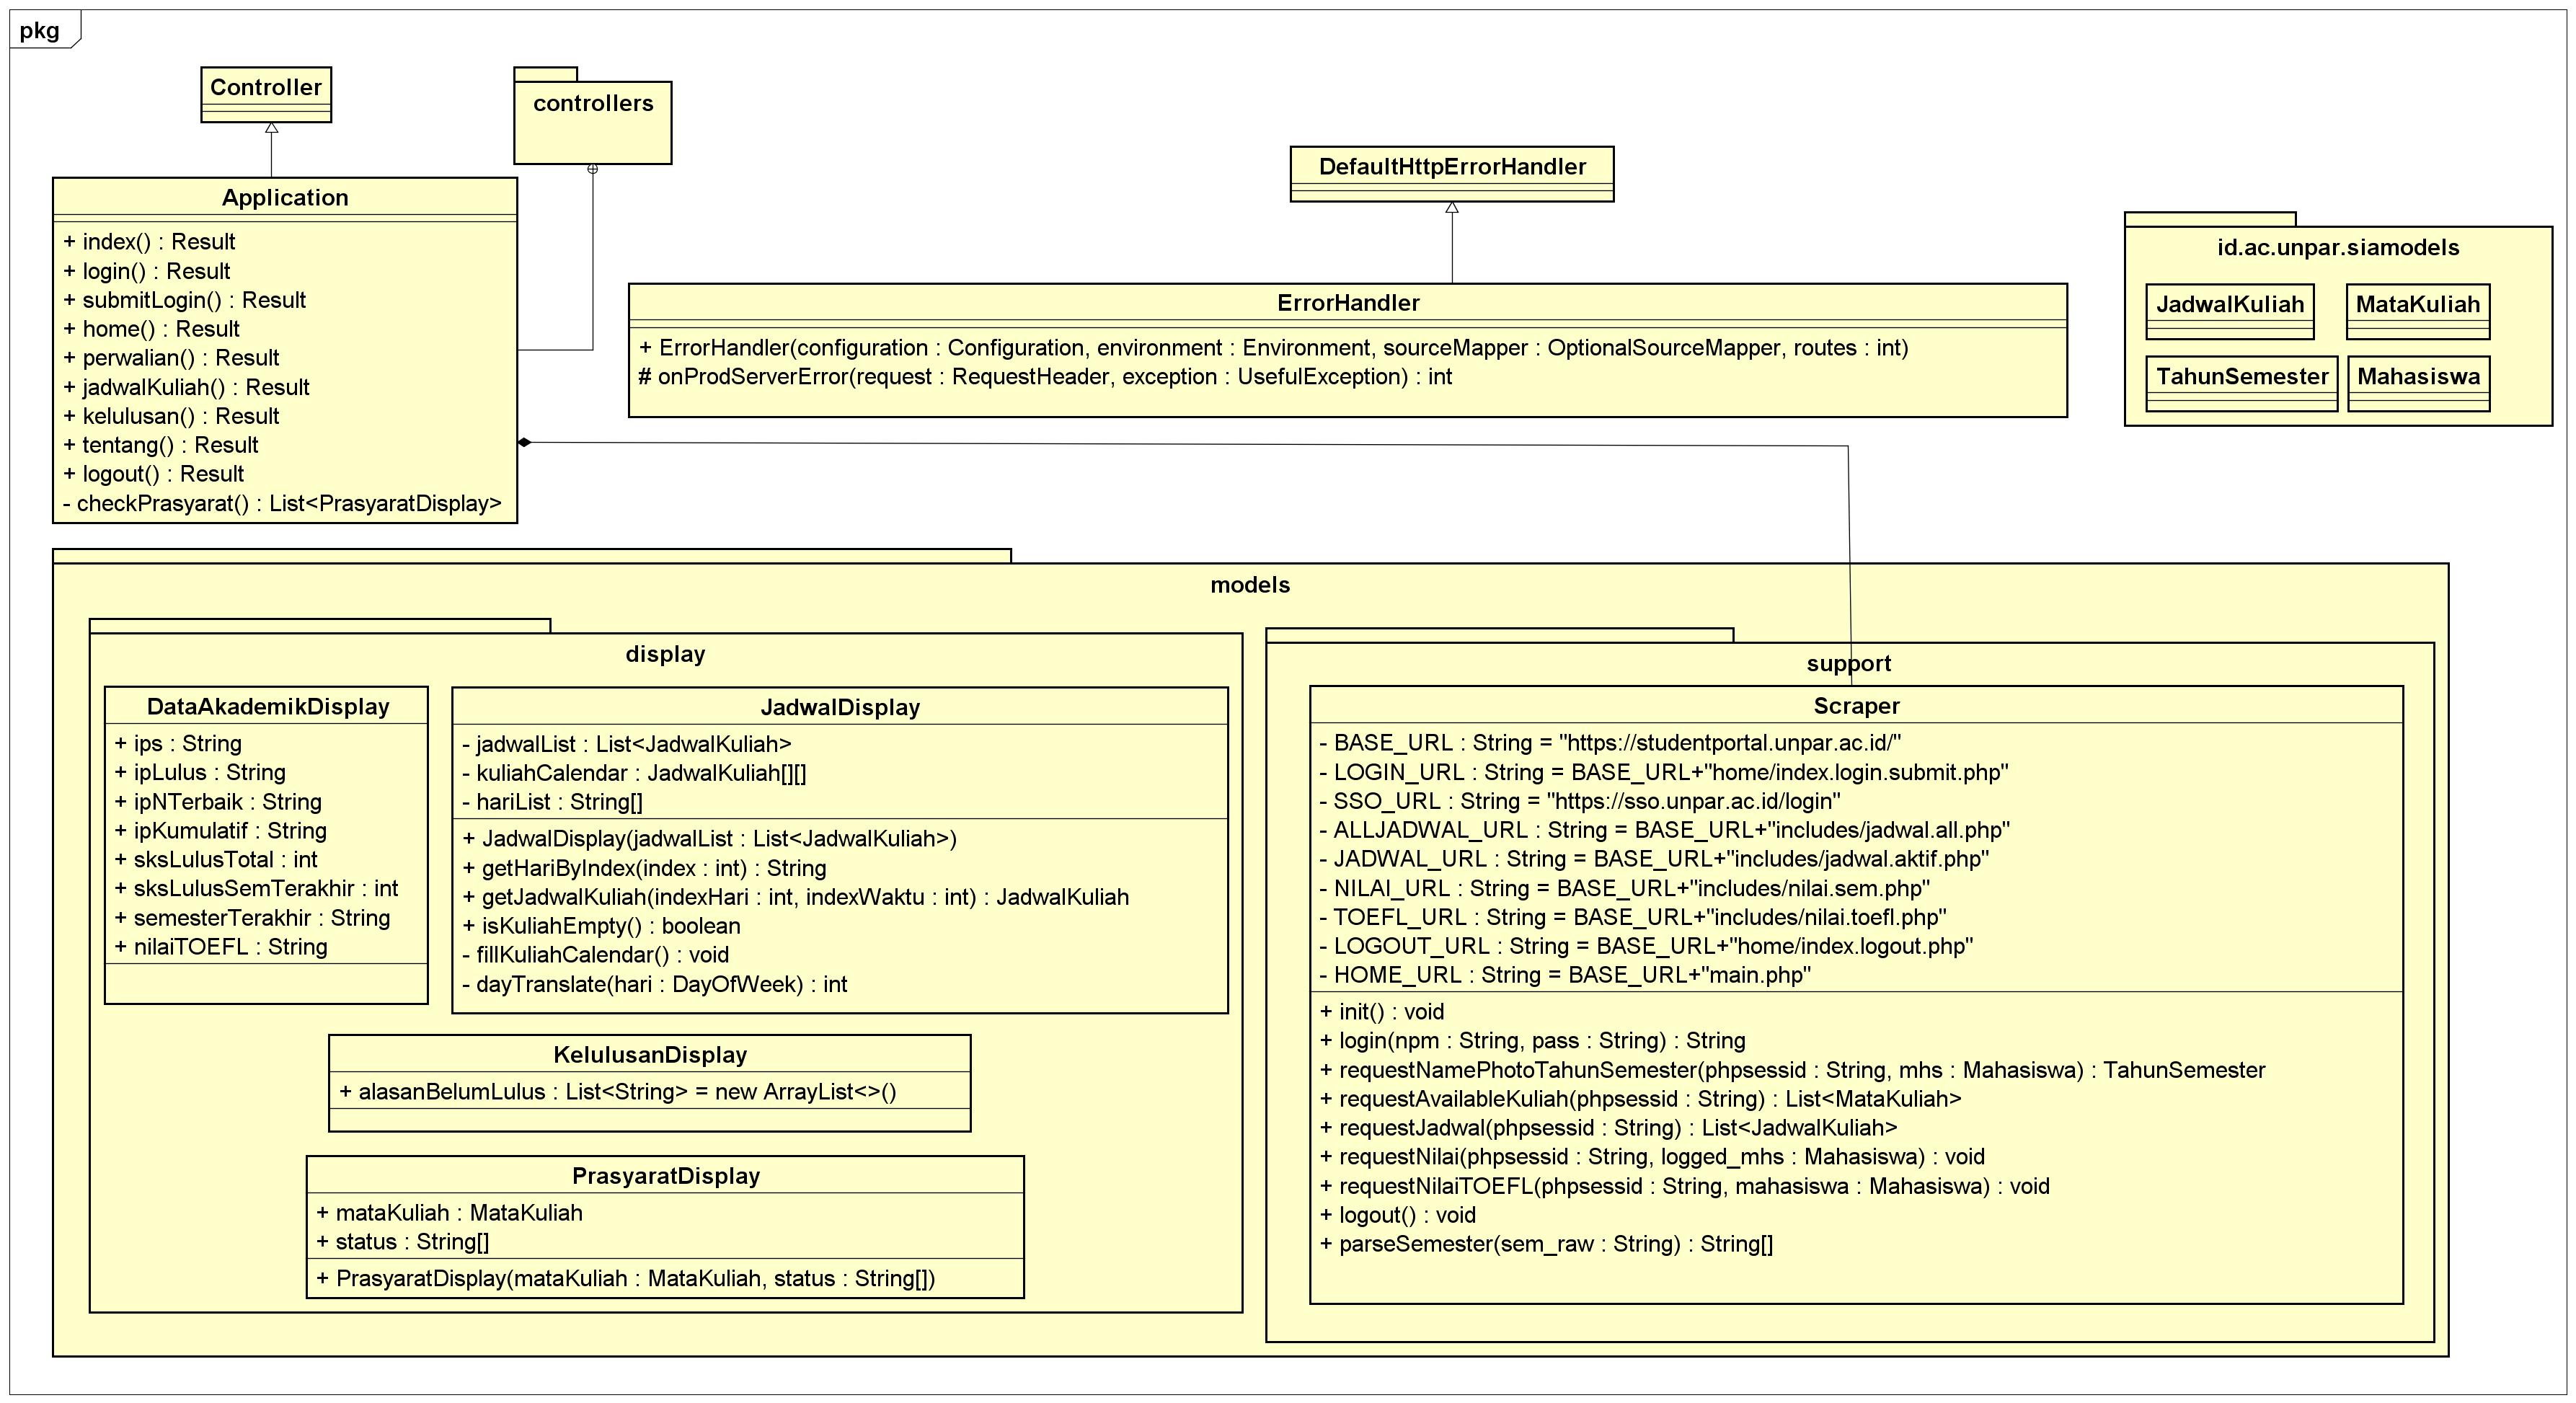
\includegraphics[scale=0.135]{Gambar/class-diagram-ifstudentportal}
\caption{Diagram Kelas IFStudentPortal}
\label{fig:2_ifstudentportal_class}
\end{figure}

\begin{enumerate}
	\item \textit{Package} \texttt{models.display}\\
	\textit{Package} ini memiliki kelas-kelas sebagai berikut:
	\begin{enumerate}
		\item DataAkademikDisplay\\
		kelas ini berfungsi sebagai media pengiriman data ke ringkasan data akademik yang berada pada halaman persiapan perwalian. Atribut yang dimiliki kelas ini antara lain:
		\begin{itemize}
			\item \textbf{String ips} IPS mahasiswa.
			\item \textbf{String ipLulus} IP Lulus mahasiswa.
			\item \textbf{String ipNTerbaik} IP N. Terbaik mahasiswa.
			\item \textbf{String ipKumulatif} IP Kumulatif mahasiswa.
			\item \textbf{int sksLulusTotal} total sks lulus mahasiswa.
			\item \textbf{int sksLulusSemTerakhir} sks lulus mahasiswa pada semester terakhir.
			\item \textbf{String semesterTerakhir} semester terakhir yang telah ditempuh mahasiswa.
			\item \textbf{String nilaiTOEFL} nilai TOEFL mahasiswa.
		\end{itemize}
		\item JadwalDisplay\\
		kelas ini berfungsi sebagai media pengiriman data ke halaman jadwal kuliah. Atribut yang dimiliki kelas ini antara lain:
		\begin{itemize}
			\item \textbf{List<JadwalKuliah> jadwalList} daftar jadwal kuliah mahasiswa. 
			\item \textbf{JadwalKuliah[][] kuliahCalendar} jadwal kuliah mahasiswa dalam \textit{array}.
			\item \textbf{String[] hariList} nama-nama hari dalam String.
		\end{itemize}
		\textit{Method-method} yang dimiliki kelas ini adalah sebagai berikut:
		\begin{itemize}
			\item \textbf{public JadwalDisplay(List<JadwalKuliah> jadwalList)}\\
			Merupakan \textit{constructor} dari kelas JadwalDisplay.\\
			\textbf{Parameter:}
			\begin{itemize}
				\item \textbf{jadwalList} jadwal kuliah mahasiswa.
			\end{itemize}
			
			\item \textbf{public String getHariByIndex(int index)}\\
			Berfungsi untuk mendapatkan hari berdasarkan angka index. Angka index dimulai dari 0 sedangkan hari dimulai dari Senin.\\
			\textbf{Parameter:}
			\begin{itemize}
				\item \textbf{index} angka index hari.
			\end{itemize}
			\textbf{Kembalian:} hari dalam String.
			
			\item \textbf{public String getJadwalKuliah(int indexHari, int indexWaktu)}\\
			Berfungsi untuk mendapatkan jadwal kuliah dari atribut kuliahCalendar.\\
			\textbf{Parameter:}
			\begin{itemize}
				\item \textbf{indexHari} angka index hari.
				\item \textbf{indexWaktu} angka index waktu.
			\end{itemize}
			\textbf{Kembalian:} jadwal kuliah.
			
			\item \textbf{public boolean isKuliahEmpty()}\\
			Berfungsi untuk memeriksa apakah nilai dari jadwal kuliah kosong.\\
			\textbf{Kembalian:} \texttt{true} jika kosong, \texttt{false} jika tidak kosong.
			
			\item \textbf{private void fillKuliahCalendar()}\\
				Berfungsi untuk mengisi atribut kuliahCalendar berdasarkan atribut jadwalList.\\
				\textbf{Kembalian:} tidak ada.
		\end{itemize}
		
		\item KelulusanDisplay\\
		Kelas ini berfungsi sebagai media pengiriman data ke halaman syarat kelulusan.Atribut yang dimiliki kelas ini antara lain:
		\begin{itemize}
			\item \textbf{List<String> alasanBelumLulus} daftar syarat kelulusan yang belum dipenuhi. 
		\end{itemize}
		\item PrasyaratDisplay\\
		Kelas ini berfungsi sebagai media pengiriman data ke halaman persiapan perwalian.Atribut yang dimiliki kelas ini antara lain:
		\begin{itemize}
			\item \textbf{MataKuliah matakuliah} mata kuliah.
			\item \textbf{String[] status} status pengambilan mata kuliah.
		\end{itemize}
	\end{enumerate}
	\item \textit{Package} \texttt{models.support}\\
	\textit{Package} ini memeliki kelas sebagai berikut:
	\begin{enumerate}
		\item Scrapper\\
		Kelas ini mengimplementasikan \textit{library} jsoup untuk melakukan pengambilan data dari Portal Akademik Mahasiswa. Atribut yang dimiliki kelas ini antara lain:
		\begin{itemize}
				\item \textbf{String BASE\_URL:} URL Portal Akademik Mahasiswa.
				\item \textbf{String LOGIN\_URL:} URL \textit{login} Portal Akademik Mahasiswa.
				\item \textbf{String SSO\_URL:} URL \textit{login} SSO UNPAR.
				\item \textbf{String ALLJADWAL\_URL:} URL jadwal seluruh fakultas pada Portal Akademik Mahasiswa.
				\item \textbf{String JADWAL\_URL:} URL jadwal mahasiswa pada Portal Akademik Mahasiswa.
				\item \textbf{String NILAI\_URL:} URL riwayat nilai mahasiswa pada Portal Akademik Mahasiswa.
				\item \textbf{String TOEFL\_URL:} URL nilai TOEFL mahasiswa pada Portal Akademik Mahasiswa.
				\item \textbf{String LOGOUT\_URL:} URL \textit{logout} Portal Akademik Mahasiswa.
				\item \textbf{HOME\_URL:} URL tampilan awal Portal Akademik Mahasiswa.
		\end{itemize}
		\textit{Method-method} yang dimiliki kelas ini adalah sebagai berikut:
		\begin{itemize}
				\item \textbf{public void init()}\\
				Berfungsi untuk menginisialisasi koneksi ke Portal Akademik Mahasiswa.\\
				\textbf{Kembalian:} tidak ada.
				
				\item \textbf{public String login(String npm, String pass)}\\
					Berfungsi untuk melakukan \textit{login}.\\
					\textbf{Parameter:}
					\begin{itemize}
						\item \textbf{npm} NPM mahasiswa.
						\item \textbf{pass} \textit{password} mahasiswa.
					\end{itemize}
					\textbf{Kembalian:} objek Mahasiswa.
			
				\item \textbf{public TahunSemester requestNamePhotoTahunSemester(String phpsessid, Mahasiswa mhs)}\\
					Berfungsi untuk melakukan permintaan nama photo pada tahun semester mahasiswa.\\
					\textbf{Parameter:}
					\begin{itemize}
						\item \textbf{phpsessid} \textit{session id} mahasiswa yang telah \textit{login}.
						\item \textbf{mhs} objek Mahasiswa.
					\end{itemize}
					\textbf{Kembalian:} objek TahunSemester.
			
				\item \textbf{public List<MataKuliah> requestAvailableKuliah(String phpsessid)}\\
					Berfungsi untuk mendapatkan daftar mata kuliah yang dibuka pada semester terkini.\\
					\textbf{Parameter:}
					\begin{itemize}
						\item \textbf{phpsessid} \textit{session id} mahasiswa yang telah \textit{login}.
					\end{itemize}
					\textbf{Kembalian:} daftar mata kuliah yang dibuka pada semester terkini.
			
				\item \textbf{public List<JadwalKuliah> requestJadwal(String phpsessid)}\\
					Berfungsi untuk mendapatkan jadwal kuliah mahasiswa pada semester terkini.\\
					\textbf{Parameter:}
					\begin{itemize}
						\item \textbf{phpsessid} \textit{session id} mahasiswa yang telah \textit{login}.
					\end{itemize}
					\textbf{Kembalian:} jadwal kuliah mahasiswa pada semester terkini.
				
					\item \textbf{public void requestNilai(String phpsessid, Mahasiswa logged\_mhs)}\\
					Berfungsi untuk mendapatkan riwayat nilai mahasiswa.\\
					\textbf{Parameter:}
					\begin{itemize}
						\item \textbf{phpsessid} \textit{session id} mahasiswa yang telah \textit{login}.
						\item \textbf{logged\_mhs} objek Mahasiswa dari mahasiswa yang telah \textit{login}.
					\end{itemize}
					\textbf{Kembalian:} tidak ada.
				
				\item \textbf{public void requestNilaiTOEFL(String phpsessid, Mahasiswa mahasiswa)}\\
					Berfungsi untuk mendapatkan riwayat nilai terakhir TOEFL mahasiswa.\\
					\textbf{Parameter:}
					\begin{itemize}
						\item \textbf{phpsessid} \textit{session id} mahasiswa yang telah \textit{login}.
						\item \textbf{mahasiswa} objek Mahasiswa dari mahasiswa yang telah \textit{login}.
					\end{itemize}
					\textbf{Kembalian:} tidak ada.
			
				\item \textbf{public void logout()}\\
					Berfungsi untuk melakukan \textit{logout}.\\
					\textbf{Kembalian:} tidak ada.
				
				\item \textbf{public String[] parseSemester(String sem\_raw)}\\
				Berfungsi untuk melakukan \textit{parsing} pada semester.\\
				\textbf{Parameter:}
					\begin{itemize}
						\item \textbf{sem\_raw} semester yang belum di parsing dalam String.
					\end{itemize}
					\textbf{Kembalian:} Semester yang sudah di parsing dalam \textit{array}.
			\end{itemize}
	\end{enumerate}
	\item \textbf{Package} \texttt{controllers}\\
	\textit{Package} ini memiliki kelas sebagai berikut:
	\begin{enumerate}
		\item Application\\
		Kelas ini merupakan turunan dari kelas Controller yang dimiliki oleh Play Framework sehingga menjadikan kelas ini sebagai controller dari aplikasi IFStudentPortal. \textit{Method-method} yang dimiliki kelas merupakan \textit{action method} dengan rincian sebagai berikut:
		\begin{itemize}
			\item \textbf{public Result index()}\\
				Berfungsi untuk mengarahkan pengguna ke halaman Informatika Student Portal.\\
				\textbf{Kembalian:} halaman \textit{login} jika pengguna belum \textit{login} atau halaman utama jika pengguna sudah \textit{login}.
				
				\item \textbf{public Result login()}\\
				Berfungsi untuk mengarahkan pengguna ke halaman \textit{login}.\\
				\textbf{Kembalian:} halaman \textit{login} jika pengguna belum \textit{login} atau halaman utama jika pengguna sudah \textit{login}.
				
				\item \textbf{public Result submitLogin()}\\
				Berfungsi untuk mengirimkan data dari halaman \textit{login} sekaligus melakukan validasi akun.\\
				\textbf{Kembalian:} halaman utama jika \textit{login} berhasil atau halaman \textit{login} jika \textit{login} gagal.
				
				\item \textbf{public Result home()}\\
				Berfungsi untuk mengarahkan pengguna ke halaman utama.\\
				\textbf{Kembalian:} halaman utama.
				
				\item \textbf{public Result perwalian()}\\
				Berfungsi untuk mengarahkan pengguna ke halaman persiapan perwalian.\\
				\textbf{Kembalian:} halaman persiapan perwalian.
				
				\item \textbf{public Result jadwalKuliah()}\\
				Berfungsi untuk mengarahkan pengguna ke halaman jadwal kuliah.\\
				\textbf{Kembalian:} halaman jadwal kuliah.
				
				\item \textbf{public Result kelulusan()}\\
				Berfungsi untuk mengarahkan pengguna ke halaman syarat kelulusan.\\
				\textbf{Kembalian:} halaman syarat kelulusan.
				
				\item \textbf{public Result tentang()}\\
				Berfungsi untuk mengarahkan pengguna ke halaman info dan lapor bug.\\
				\textbf{Kembalian:} halaman info dan lapor bug.
				
				\item \textbf{public Result logout()}\\
				Berfungsi untuk mengeluarkan pengguna yang sedang \textit{login}.\\
				\textbf{Kembalian:} halaman \textit{login}.
				
				item \textbf{public List<PrasyaratDisplay> checkPrasyarat()}\\
				Berfungsi untuk memeriksa prasyarat dari mata kuliah yang sudah diambil mahasiswa.\\
				\textbf{Kembalian:} daftar prasyarat mata kuliah.
		\end{itemize}
	\end{enumerate}
\end{enumerate}

\section{SIAModels}
\label{sec:siamodels}

SIAModels merupakan kelas-kelas dalam bahasa Java yang merepresentasikan Sistem Informasi Akademik Teknik Informatika UNPAR \cite{siamodels}. Saat ini SIAModels mendukung kurikulum 2013. Berdasarkan diagram kelas SIAModels (Gambar \ref{fig:2_siamodels_class}), kelas-kelas yang dimiliki SIAModels terbagi ke dalam empat \textit{package} antara lain:

\begin{figure}[H]
\centering
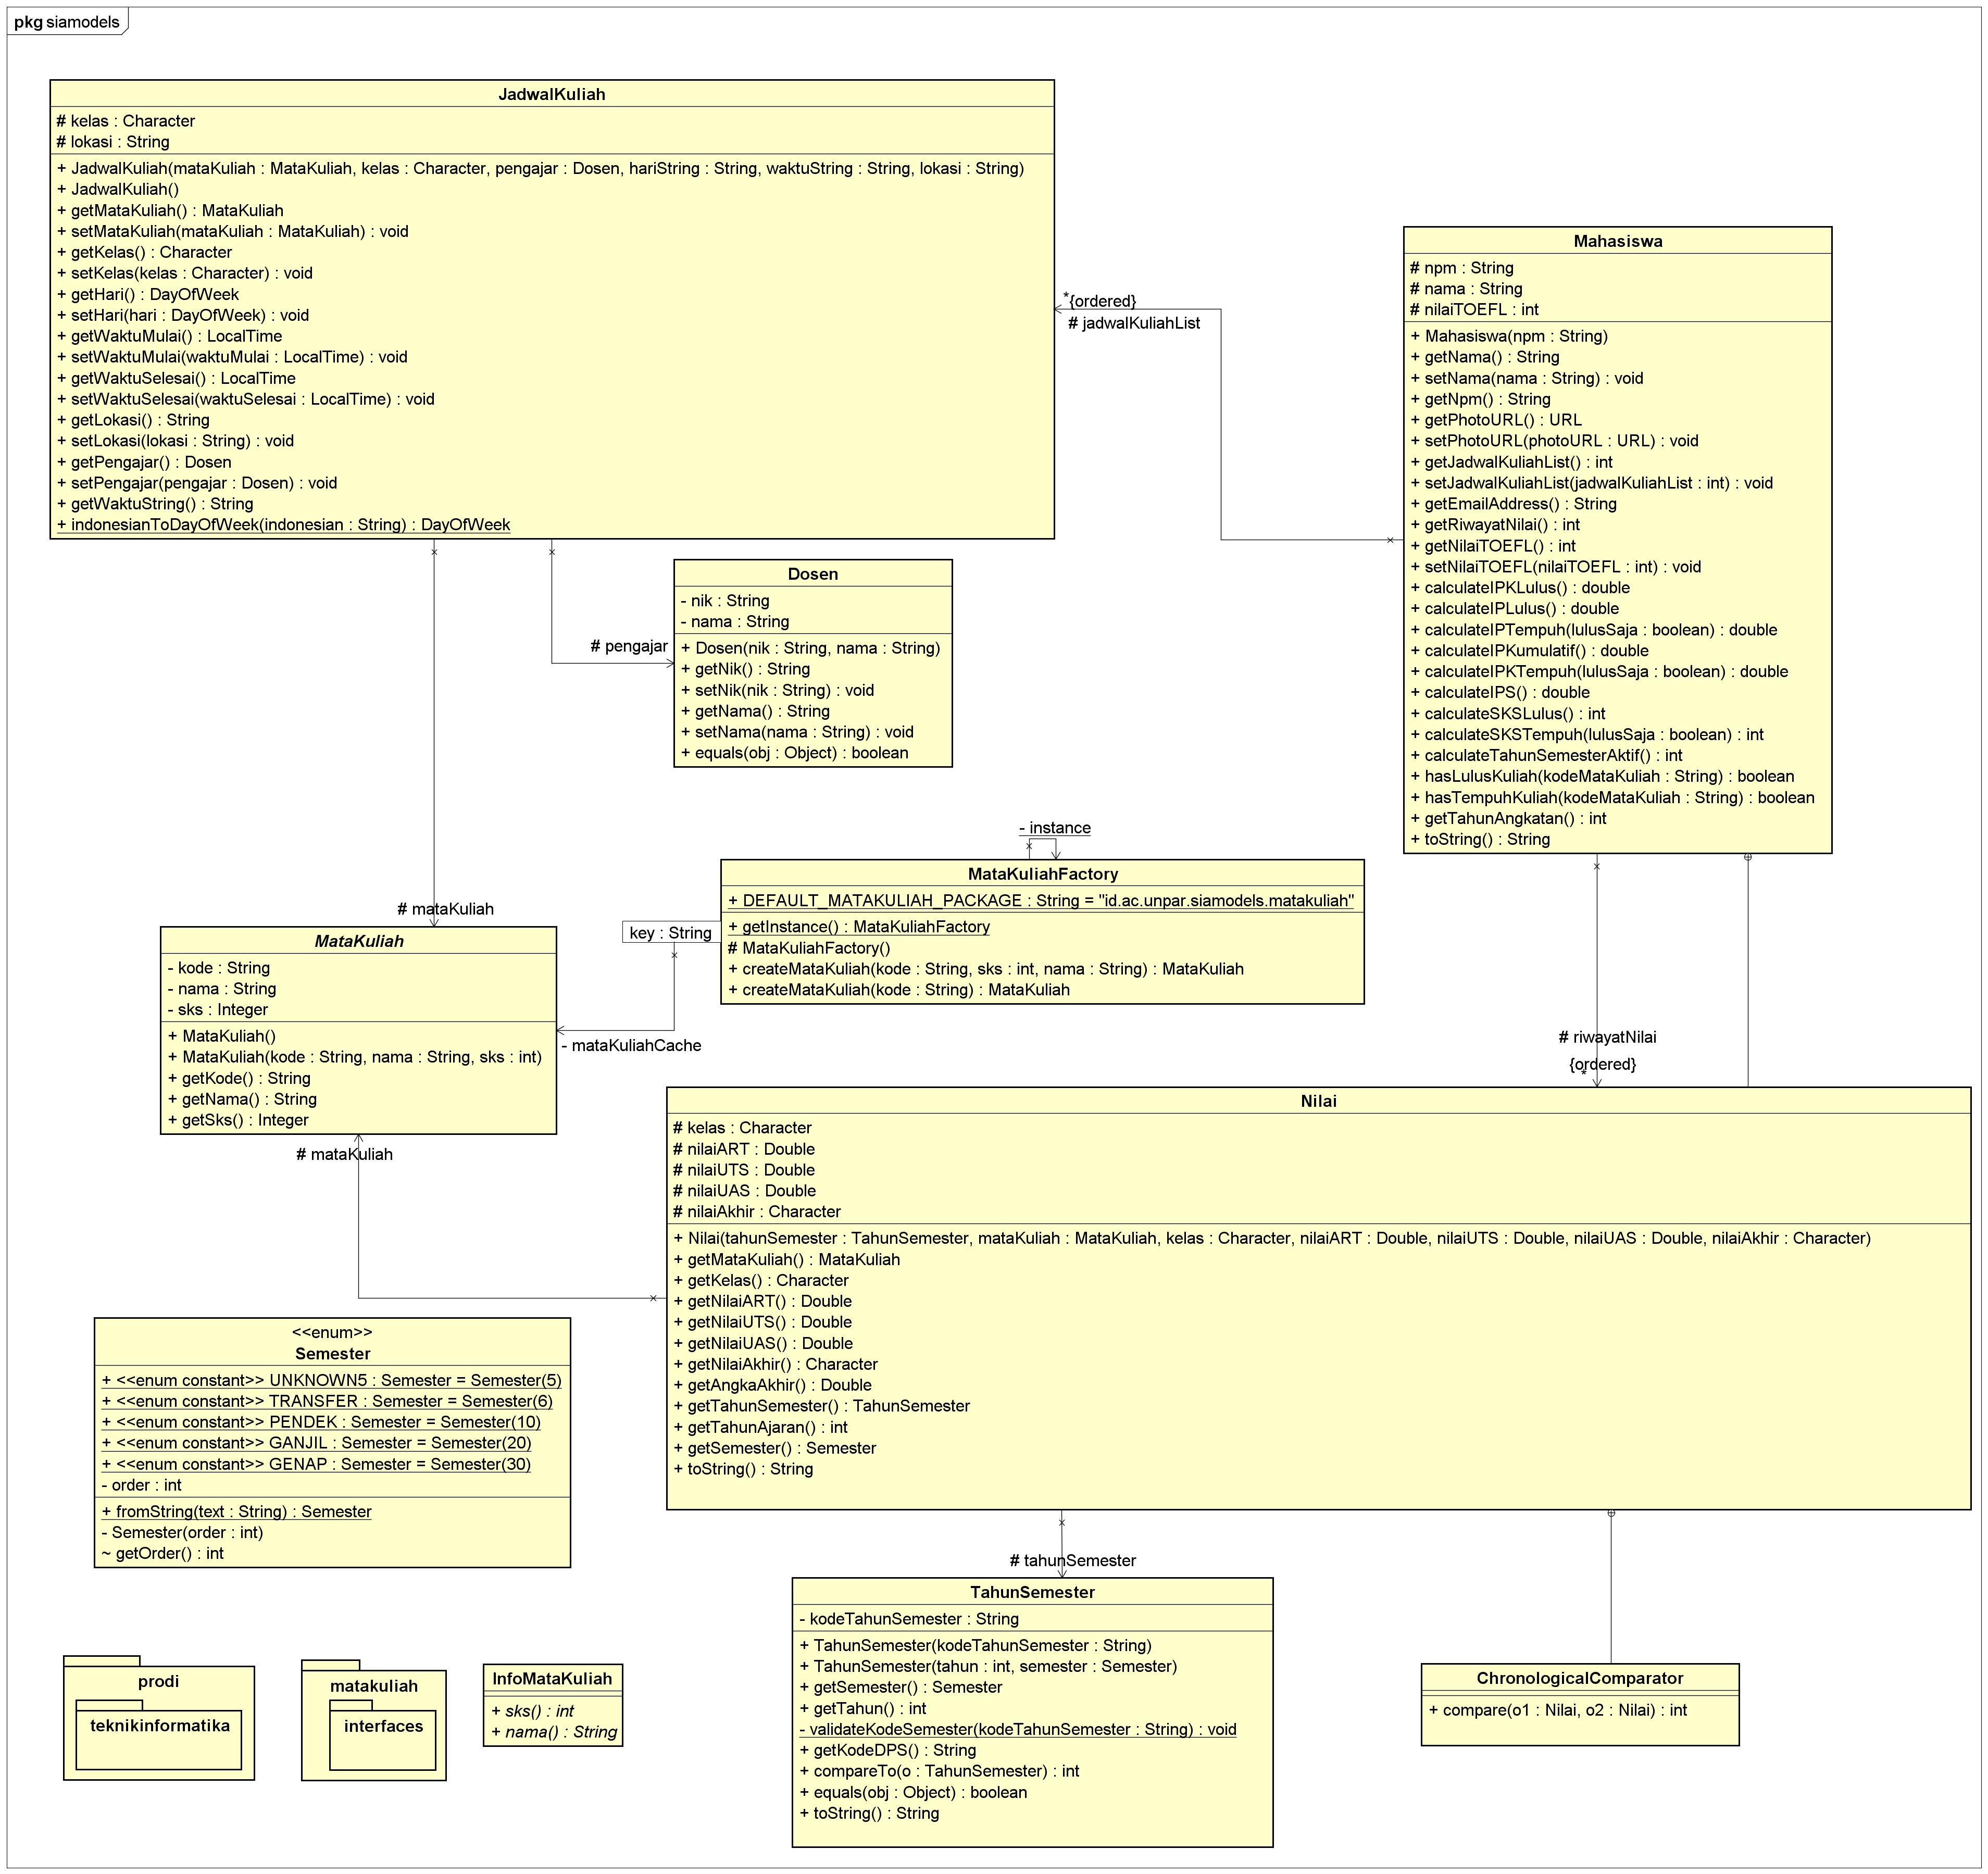
\includegraphics[scale=0.125]{Gambar/class-diagram-siamodels}
\caption{Diagram Kelas SIAModels}
\label{fig:2_siamodels_class}
\end{figure}

\begin{enumerate}
	\item \textit{Package} \texttt{id.ac.unpar.siamodels}\\
	\textit{Package} ini memiliki kelas-kelas sebagai berikut:
	\begin{enumerate}
		\item Dosen\\
		Kelas ini merepresentasikan dosen. Atribut yang dimiliki kelas ini antara lain:
		\begin{itemize}
			\item \textbf{String nik:} NIK.
			\item \textbf{String nama:} nama dosen.
		\end{itemize}
	\textit{Method-method} yang dimiliki kelas ini adalah sebagai berikut:
		\begin{itemize}
			\item \textbf{public String getNik()}\\
				Berfungsi untuk mendapatkan NIK dosen.\\
				\textbf{Kembalian:} NIK dosen.

			\item \textbf{public void setNik(String nik)}\\
				Berfungsi untuk mengubah nik dosen.\\
				\textbf{Parameter:}
				\begin{itemize}
					\item \textbf{nik} nik dosen.
				\end{itemize}
				
			\item \textbf{public String getNama()}\\
				Berfungsi untuk mendapatkan nama dosen.\\
				\textbf{Kembalian:} nama dosen.

			\item \textbf{public void setNama(String nama)}\\
				Berfungsi untuk mengubah nama dosen.\\
				\textbf{Parameter:}
				\begin{itemize}
					\item \textbf{nama} nama dosen.
				\end{itemize}
				
			\item \textbf{public boolean equals(Object obj)}\\
			Berfungsi untuk memeriksa keseteraan untuk dosen. pertama periksa NIK kalau keduanya ada. jika tidak, periksa nama.
			\textbf{Parameter:}
			\begin{itemize}
				\item \textbf{obj} objek kelas dosen yang ingin dibandingkan.
			\end{itemize}
			\textbf{Kembalian:} \texttt{true} jika setera, \texttt{false} jika tidak.
		\end{itemize}						
		
		\item InfoMataKuliah\\
		Mendefinisikan kelas-kelas yang memiliki info mata kuliah. \textit{Method} yang dimiliki \textit{interface} ini adalah sebagai berikut:
		\begin{itemize}
			\item \textbf{public int sks()}\\
			Mengetahui jumlah bobot sks dari mata kuliah ini.
			\textbf{Kembalian:} jumlah bobot sks.
			\item \textbf{public String nama()}\\
			Mengetahui nama mata kuliah ini.
			\textbf{Kembalian:} nama mata kuliah.
		\end{itemize}
		
		\item JadwalKuliah\\
		Kelas ini merepresentasikan jadwal kuliah mahasiswa. Atribut yang dimiliki kelas ini antara lain:
		\begin{itemize}
			\item \textbf{MataKuliah mataKuliah:} mata kuliah yang dibuat jadwalnya.
			\item \textbf{Character kelas:} kelas kuliah.
			\item \textbf{DayOfWeek hari:} hari kuliah.
			\item \textbf{LocalTime waktuMulai:} waktu mulai kuliah.
			\item \textbf{LocalTime waktuSelesai:} waktu selesai kuliah.
			\item \textbf{String lokasi:} kode ruangan.
			\item \textbf{Dosen pengajar:} nama pengajar.
		\end{itemize}
	\textit{Method-method} yang dimiliki kelas ini adalah sebagai berikut:
		\begin{itemize}
			\item \textbf{public MataKuliah getMataKuliah()}\\
				Berfungsi untuk mendapatkan mata kuliah yang dibuat jadwalnya.\\
				\textbf{Kembalian:} mata kuliah yang dibuat jadwalnya.

			\item \textbf{public void setMataKuliah(MataKuliah mataKuliah)}\\
				Berfungsi untuk mengubah mata kuliah yang dibuat jadwalnya.\\
				\textbf{Parameter:}
				\begin{itemize}
					\item \textbf{mataKuliah} mata kuliah yang dibuat jadwalnya.
				\end{itemize}
				
			\item \textbf{public Character getKelas()}\\
				Berfungsi untuk mendapatkan kelas kuliah.\\
				\textbf{Kembalian:} kelas kuliah.

			\item \textbf{public void setKelas(Character kelas)}\\
				Berfungsi untuk mengubah kelas kuliah.\\
				\textbf{Parameter:}
				\begin{itemize}
					\item \textbf{kelas} kelas kuliah.
				\end{itemize}
				
			\item \textbf{public DayOfWeek getHari()}\\
				Berfungsi untuk mendapatkan hari kuliah.\\
				\textbf{Kembalian:} hari kuliah.

			\item \textbf{public void setHari(DayOfWeek hari)}\\
				Berfungsi untuk mengubah hari kuliah.\\
				\textbf{Parameter:}
				\begin{itemize}
					\item \textbf{hari} hari kuliah.
				\end{itemize}
			\item \textbf{public LocalTime getWaktuMulai()}\\
				Berfungsi untuk mendapatkan waktu mulai kuliah.\\
				\textbf{Kembalian:} waktu mulai kuliah.

			\item \textbf{public void setWaktuMulai(LocalTime waktuMulai)}\\
				Berfungsi untuk mengubah waktu mulai kuliah.\\
				\textbf{Parameter:}
				\begin{itemize}
					\item \textbf{waktuMulai} waktu mulai kuliah.
				\end{itemize}
				
			\item \textbf{public void setWaktuSelesai(LocalTime waktuSelesai)}\\
				Berfungsi untuk mengubah waktu selesai kuliah.\\
				\textbf{Parameter:}
				\begin{itemize}
					\item \textbf{waktuSelesai} waktu selesai kuliah.
				\end{itemize}
			
			\item \textbf{public String getLokasi()}\\
				Berfungsi untuk mendapatkan lokasi kuliah.\\
				\textbf{Kembalian:} lokasi kuliah.

			\item \textbf{public void setLokasi(String lokasi)}\\
				Berfungsi untuk mengubah lokasi kuliah.\\
				\textbf{Parameter:}
				\begin{itemize}
					\item \textbf{lokasi} lokasi kuliah.
				\end{itemize}
				
			\item \textbf{public Dosen getPengajar()}\\
				Berfungsi untuk mendapatkan nama pengajar.\\
				\textbf{Kembalian:} nama pengajar.

			\item \textbf{public void setPengajar(Dosen Pengajar)}\\
				Berfungsi untuk mengubah nama pengajar.\\
				\textbf{Parameter:}
				\begin{itemize}
					\item \textbf{pengajar} nama pengejar.
				\end{itemize}
		\end{itemize}
		
		\item Mahasiswa\\
		Kelas ini merepresentasikan mahasiswa. Atribut yang dimiliki kelas ini antara lain:
		\begin{itemize}
			\item \textbf{String npm:} Nomor Pokok Mahasiswa (NPM).
			\item \textbf{String nama:} nama mahasiswa.
			\item \textbf{List<Nilai> riwayatNilai:} riwayat nilai 		yang dimiliki mahasiswa.
			\item \textbf{URL photoURL:} alamat dari photo mahasiswa.
			\item \textbf{List<JadwalKuliah> jadwalKuliahList:} daftar jadwal kuliah dari mahasiswa.
			\item \textbf{SortedMap<LocalDate, Integer> nilaiTOEFL:} nilai TOEFL dari mahasiswa.
		\end{itemize}
	\textit{Method-method} yang dimiliki kelas ini adalah sebagai berikut:
		\begin{itemize}
			\item \textbf{public Mahasiswa (String npm)}\\
			Merupakan \textit{constructor} dari kelas Mahasiswa.\\
			\textbf{Parameter:}
			\begin{itemize}
				\item \textbf{npm} nomor pokok mahasiswa.
			\end{itemize}
			\item \textbf{public String getNama()}\\
				Berfungsi untuk mendapatkan nama mahasiswa.\\
				\textbf{Kembalian:} nama mahasiswa.

			\item \textbf{public void setNama(String nama)}\\
				Berfungsi untuk mengubah nama mahasiswa.\\
				\textbf{Parameter:}
				\begin{itemize}
					\item \textbf{nama} nama mahasiswa.
				\end{itemize}
		
			\item \textbf{public String getNpm()}\\
				Berfungsi untuk mendapatkan nomor pokok mahasiswa.\\
				\textbf{Kembalian:} nomor pokok mahasiswa.
				
			\item \textbf{public URL getPhotoURL()}\\
				Berfungsi untuk mendapatkan alamat photo dari mahasiswa.\\
				\textbf{Kembalian:} URL dari photo
			
			\item \textbf{public void setPhotoURL(URL photoURL)}\\
				Berfungsi untuk mengubah URL photo dari mahasiswa.\\
				\textbf{Parameter:}
				\begin{itemize}
					\item \textbf{photoURL} alamat photo dari mahasiswa.
				\end{itemize}
				
			\item \textbf{public List<JadwalKuliah> getJadwalKuliahList()}\\
				Berfungsi untuk mendapatkan daftar jadwal kuliah  dari mahasiswa.\\
				\textbf{Kembalian:} daftar jadwal kuliah dari mahasiswa.
			
			\item \textbf{public void setJadwalKuliahList(List<JadwalKuliah> jadwalKuliahList)}\\
				Berfungsi untuk mengubah daftar jadwal kuliah dari mahasiswa.\\
				\textbf{Parameter:}
				\begin{itemize}
					\item \textbf{jadwalKuliahList} daftar jadwal kuliah dari mahasiswa.
				\end{itemize}
			
			\item \textbf{public String getEmailAddress()}\\
				Berfungsi untuk mendapatkan \textit{email} mahasiswa.\\
				\textbf{Kembalian:} \textit{email} mahasiswa.
				
			\item \textbf{public List<Nilai> getRiwayatNilai()}\\
				Berfungsi untuk mendapatkan riwayat nilai mahasiswa.\\
				\textbf{Kembalian:} riwayat nilai mahasiswa dalam List.
			\item \textbf{public SortedMap<LocalDate, Integer> getNilaiTOEFL()}\\
				Berfungsi untuk mendapatkan nilai TOEFL  dari mahasiswa.\\
				\textbf{Kembalian:} nilai TOEFL dari mahasiswa.
			
			\item \textbf{public void setNilaiTOEFL(SortedMAP<LocalDate, Integer> nilaiTOEFL)}\\
				Berfungsi untuk mengubah nilai TOEFL dari mahasiswa.\\
				\textbf{Parameter:}
				\begin{itemize}
					\item \textbf{nilaiTOEFL} nilai TOEFL dari mahasiswa.
				\end{itemize}
			 
			 \item \textbf{public double calculateIPKLulus()}\\
				Menghitung IPK mahasiswa sampai saat ini, dengan aturan kuliah yang tidak lulus tidak dihitung dan jika pengambilan beberapa kali, diambil nilai terbaik. Sebelum memanggil \textit{method} ini, \texttt{getRiwayatNilai()} harus sudah mengandung nilai per mata kuliah.\\
				\textbf{Kembalian:} IPK lulus.
			
			\item \textbf{public double calculateIPLulus()}\\
				Menghitung IP mahasiswa sampai saat ini, dengan aturan kuliah yang tidak lulus tidak dihitung, jika pengembalian beberapa kali, maka diambil nilai terbaik. Sebelum memanggil \textit{method} ini, \texttt{getRiwayatNilai()} harus sudah mengandung nilai per mata kuliah.\\
				\textbf{Kembalian:}  IPK lulus.
			
			\item \textbf{public double calculateIPTempuh(boolean lulusSaja)}\\
				Menghitung IP mahasiswa sampai saat ini, dengan aturan perhitungan kuliah yang tidak lulus ditentukan parameter, jika pengembilan beberapa kali, maka diambil nilai terbaik. Sebelum memanggil \textit{method} ini, \texttt{getRiwayatNilai()} harus sudah mengandung nilai per mata kuliah.\\
				\textbf{Parameter:} 
				\begin{itemize}
					\item \textbf{lulusSaja} \texttt{true} jika ingin membuang mata kuliah tidak lulus, \texttt{false} jika ingin semua (sama dengan "IP N. Terbaik" di DPS)
				\end{itemize}
				\textbf{Kembalian:}  IPK lulus.
			
			\item \textbf{public double calculateIPKumulatif()}\\
				Menghitung IP Kumulatif mahasiswa sampai saat ini, dengan aturan jika pengembalian beberapa kali, maka diambil semua. Sebelum memanggil \textit{method} ini, \texttt{getRiwayatNilai()} harus sudah mengandung nilai per mata kuliah.\\
				\textbf{Kembalian:}  IPK lulus.
				
						\item \textbf{public double calculateIPKTempuh(boolean lulusSaja)}\\
				Menghitung IPK mahasiswa sampai saat ini, dengan aturan perhitungan kuliah yang tidak lulus ditentukan parameter, jika pengembilan beberapa kali, maka diambil nilai terbaik. Sebelum memanggil \textit{method} ini, \texttt{getRiwayatNilai()} harus sudah mengandung nilai per mata kuliah.\\
				\textbf{Parameter:} 
				\begin{itemize}
					\item \textbf{lulusSaja} \texttt{true} jika ingin membuang mata kuliah tidak lulus
				\end{itemize}
				\textbf{Kembalian:}  IPK lulus.
			
			\item \textbf{public double calculateIPS()}\\
				Menghitung IPS semester terakhir sampai saat ini, dengan aturan kuliah yang tidak lulus dihitung. Sebelum memanggil \textit{method} ini, \texttt{getRiwayatNilai()} harus sudah mengandung nilai per mata kuliah.\\
				\textbf{Kembalian:}  nilai IPS sampai saat ini.
				
			\item \textbf{public int calculateSKSLulus()}\\
				Menghitung jumlah SKS lulus mahasiswa saat ini. Sebelum memanggil \textit{method} ini, \texttt{getRiwayatNilai()} harus sudah mengandung nilai per mata kuliah.\\
				\textbf{Kembalian:} SKS lulus.
			
			\item \textbf{public int calculateSKSTempuh(boolean lulusSaja)}\\
				Menghitung jumlah SKS lulus mahasiswa saat ini. Sebelum memanggil \textit{method} ini, \texttt{getRiwayatNilai()} harus sudah mengandung nilai per mata kuliah.\\
				\textbf{Parameter:} 
				\begin{itemize}
					\item \textbf{lulusSaja} \texttt{true} jika ingin membuang SKS tidak lulus.
				\end{itemize}
				\textbf{Kembalian:} SKS tempuh.
				
			\item \textbf{public Set<TahunSemester> calculateTahunSemesterAktif()}\\
				Mendapatkan seluruh tahun semester di mana mahasiswa ini tercatat sebagai mahasiswa aktif, dengan strategi memeriksa riwayat nilainya.Jika ada satu nilai saja pada sebuah tahun semester, maka dianggap aktif pada semester tersebut.\\
				\textbf{Kembalian:} kumpulan tahun semester di mana mahasiswa ini aktif.
			
			\item \textbf{public boolean hasLulusKuliah(String kodeMataKuliah)}\\
				Memeriksa apakah mahasiswa ini sudah lulus mata kuliah tertentu. Sebelum memanggil \textit{method} ini, \texttt{getRiwayatNilai()} harus sudah mengandung nilai per mata kuliah.\\
				\textbf{Parameter:}
				\begin{itemize}
					\item \textbf{kodeMataKuliah} kode mata kuliah yang ingin diperiksa kelulusannya.
				\end{itemize}
				\textbf{Kembalian:} \texttt{true} jika sudah pernah mengambil dan lulus, \texttt{false} jika belum.
				
			\item \textbf{public boolean hasTempuhKuliah(String kodeMataKuliah)}\\
				Memeriksa apakah mahasiswa ini sudah pernah menempuh mata kuliah tertentu. Sebelum memanggil \textit{method} ini, \texttt{getRiwayatNilai()} harus sudah mengandung nilai per mata kuliah.\\
				\textbf{Parameter:}
				\begin{itemize}
					\item \textbf{kodeMataKuliah} kode mata kuliah yang ingin diperiksa kelulusannya.
				\end{itemize}
				\textbf{Kembalian:} \texttt{true} jika sudah pernah mengambil, \texttt{false} jika belum.
				
			\item \textbf{public int getTahunAngkatan()}\\
				Mendapatkan tahun angkatan mahasiswa ini berdasarkan NPM-nya.\\
				\textbf{Kembalian:} tahun angkatan.
		\end{itemize}
		
		\item Nilai\\
		Kelas ini merepresentasikan nilai yang ada pada riwayat nilai mahasiswa. Atribut yang dimiliki kelas ini antara lain:
		\begin{itemize}
			\item \textbf{TahunSemester tahunSemester:} tahun dan semester kuliah ini diambil
			\item \textbf{MataKuliah mataKuliah:} mata kuliah yang diambil.
			\item \textbf{Character kelas:} kelas kuliah.
			\item \textbf{Double nilaiART:} nilai Angka Rata-rata Tugas (ART).
			\item \textbf{Double nilaiUTS:} nilai Ujian Tengah Semester (UTS).
			\item \textbf{Double nilaiUAS:} nilai Ujian Akhir Semester (UAS).
			\item \textbf{Character nilaiAkhir:} nilai akhir.
		\end{itemize}
	\textit{Method-method} yang dimiliki kelas ini adalah sebagai berikut:
		\begin{itemize}
			\item \textbf{public Nilai(TahunSemester tahunSemester, MataKuliah mataKuliah, Character kelas, Double nilaiART, Double nilaiUTS, Double nilaiUAS, Character nilaiAkhir)}\\
				Merupakan \textit{constructor} dari kelas Nilai.\\
				\textbf{Parameter:}
				\begin{itemize}
					\item \textbf{tahunSemester} tahun dan semester kuliah ini diambil.
					\item \textbf{mataKuliah} mata kuliah yang diambil.
					\item \textbf{kelas} kelas kuliah.
					\item \textbf{nilaiART} nilai ART.
					\item \textbf{nilaiUTS} nilai UTS.
					\item \textbf{nilaiUAS} nilai UAS.
					\item \textbf{nilaiAkhir} nilai akhir.
				\end{itemize}
				
			\item \textbf{public MataKuliah getMataKuliah()}\\
				Mendapatkan mata kuliah yang diambil.\\
				\textbf{Kembalian:} mata kuliah.
				
			\item \textbf{public Character getKelas()}\\
				Mendapatkan kelas kuliah.\\
				\textbf{Kembalian:} kelas kuliah.
				
			\item \textbf{public Double getNilaiART()}\\
				Mendapatkan nilai ART.\\
				\textbf{Kembalian:} nilai ART.
				
			\item \textbf{public Double getNilaiUTS()}\\
				Mendapatkan nilai UTS.\\
				\textbf{Kembalian:} nilai UTS.
				
			\item \textbf{public Double getNilaiUAS()}\\
				Mendapatkan nilai UAS.\\
				\textbf{Kembalian:} nilai UAS.
				
			\item \textbf{public Character getNilaikhir()}\\
				Mengembalikan nilai akhir dalam bentuk huruf (A, B, C, D, ...).\\
				\textbf{Kembalian:} nilai akhir dalam huruf atau \texttt{null} jika tidak ada.
			
			\item \textbf{public Double getAngkaAkhir()}\\
				Mendapatkan nilai akhir dalam bentuk angka.\\
				\textbf{Kembalian:} nilai akhir dalam angka, atau \texttt{null} jika \texttt{getNilaiAkhir()} mengembalikan \texttt{null}.
			
			\item \textbf{public int getTahunAjaran()}\\
				Mendapatkan tahun ajaran saat pengambilan mata kuliah.\\
				\textbf{Kembalian:} tahun ajaran saat pengambilan mata kuliah.
			
			\item \textbf{public TahunSemester getTahunSemester()}\\
				Mendapatkan tahun dan semester pengambilan mata kuliah.\\
				\textbf{Kembalian:} tahun dan semester pengambilan mata kuliah.	
				
			\item \textbf{public Semester getSemester()}\\
				Mendapatkan semester pengambilan mata kuliah.\\
				\textbf{Kembalian:} semester pengambilan mata kuliah
		\end{itemize}
		
		\item ChronologicalComparator\\
		Pembanding antara satu nilai dengan nilai lainnya, secara kronologis waktu pengambilan. \textit{Method} yang dimiliki kelas ini adalah sebagai berikut:
		
		\begin{itemize}
			\item \textbf{public int compare(Nilai o1, Nilai o2) } \\
			Berfungsi untuk membandingkan nilai. \\
			\textbf{Parameter:}
			\begin{itemize}
				\item \textbf{o1} nilai pertama yang akan dibandingkan.
				\item \textbf{o2} nilai kedua yang akan dibandingkan.
			\end{itemize}
			\textbf{Kembalian:} hasil perbandingan.
		\end{itemize}
		
		\item MataKuliah\\
		Kelas ini merepresentasikan sebuah mata kuliah.\textit{Method-method} yang dimiliki kelas ini adalah sebagai berikut:	
		\begin{itemize}
			\item \textbf{public String kode()} \\
			Mendapatkan kode mata kuliah sesuai dengan nama kelas mata kuliah tersebut. \\
			\textbf{Kembalian:} kode mata kuliah.
			\item \textbf{public int sks()} \\
			Mendapatkan bobot sks. \\
			\textbf{Kembalian:} bobot SKS.
			\item \textbf{public String kode()} \\
			Mendapatkan nama mata kuliah. \\
			\textbf{Kembalian:} nama mata kuliah.
		\end{itemize}
		
		\item MataKuliahFactory\\
		Kelas ini berperan dalam pembuatan objek mata kuliah baru. Atribut yang dimiliki kelas ini antara lain:
		\begin{itemize}
			\item \textbf{String DEFAULT\_MATAKULIAH\_PACKAGE:} lokasi \textit{package} untuk daftar mata kuliah.
			\item \textbf{MataKuliahFacory isntance:} \textit{Singleton instance} untuk \textit{factory}.
			\item \textbf{SortedMap<String, MataKuliah> mataKuliahCache:} \textit{Singleton instances} untuk mata kuliah.
		\end{itemize}
		\textit{Method} yang dimiliki kelas ini adalah sebagai berikut:
		\begin{itemize}	
			\item \textbf{public static MataKuliah createMataKuliah(String kode, int sks, String nama)} \\
			Membuat objek mata kuliah baru. Jika memungkinkan mengambil dari kelas yang sudah ada.\\
			\textbf{Parameter:}
			\begin{itemize}
				\item \textbf{kode} kode mata kuliah.
				\item \textbf{sks} bobot SKS mata kuliah.
				\item \textbf{nama} nama mata kuliah.
			\end{itemize}
			\textbf{Kembalian:} objek mata kuliah.
		\end{itemize}
		
		\item Semester\\
		Kelas ini merepresentasikan semester
		\textit{Method} yang dimiliki kelas ini adalah sebagai berikut:
		\begin{itemize}
			\item \textbf{public static final Semester fromString(String text)} \\
			Berfungsi untuk mengubah semester dari bentuk teks ke konstanta. \\
			\textbf{Parameter:}
			\begin{itemize}
				\item \textbf{text} semester dalam bentuk teks (GANJIL, GENAP, PENDEK, TRANSFER, dan UNKNOWN5).
			\end{itemize}
			\textbf{Kembalian:} konstanta semester.
		\end{itemize}
		
		\item TahunSemester\\
		Kelas ini menyimpan konstanta untuk semester beserta tahunnya di UNPAR. Atribut yang dimiliki kelas ini antara lain:
		\begin{itemize}
			\item \textbf{String kodeTahunSemester:} kode semester 3 dijit, 2 dijit pertama berupa tahun, dijit terakhir menandakan semester dengan definisi 1 untuk ganjil, 2 untuk genap, 4 untuk pendek, dan 6 untuk transfer.
		\end{itemize}
		\textit{Method-method} yang dimiliki kelas ini adalah sebagai berikut:
		\begin{itemize}
			\item \textbf{public TahunSemester(String kodeTahunSemester)} \\
			\textit{Method} ini merupakan constructor dari kelas TahunSemester. \\
			\textbf{Parameter:}
			\begin{itemize}
				\item \textbf{kodeTahunSemester} semester dalam bentuk teks (GANJIL, GENAP, PENDEK, TRANSFER, dan UNKNOWN5).
			\end{itemize}
			
			\item \textbf{public TahunSemester(int tahun, Semester semester)} \\
			\textit{Method} ini merupakan constructor dari kelas TahunSemester. \\
			\textbf{Parameter:}
			\begin{itemize}
				\item \textbf{tahun} tahun ajaran.
				\item \textbf{semester} semester dari tahun ajaran.
			\end{itemize}
			
			\item \textbf{public Semester getSemester()} \\
			\textit{Method} ini berfungsi untuk mendapatkan semester. \\
			\textbf{Kembalian:} semester dalam teks.
			
			\item \textbf{public int getTahun()} \\
			\textit{Method} ini berfungsi untuk mendapatkan tahun. \\
			\textbf{Kembalian:} tahun ajaran.
			
			\item \textbf{private static void validateKodeSemester(String kodeTahunSemester)} \\
			\textit{Method} ini berfungsi untuk melakukan  validasi terhadap kode tahun semester. \\
			\textbf{Parameter:}
			\begin{itemize}
				\item \textbf{kodeTahunSemester} kode tahun semester.
			\end{itemize}
		\end{itemize}
	\end{enumerate}
	\item \textit{Package} \texttt{id.ac.unpar.siamodels.matakuliah.interfaces}\\
	\textit{Package} ini memiliki beberapa \textit{interface} antara lain:
	\begin{enumerate}
		\item HasPrasyarat\\
		Mendefinisikan kelas-kelas yang memiliki prasyarat, terkustomisasi untuk seorang mahasiswa. \textit{Method} yang dimiliki \textit{interface} ini adalah sebagai berikut:
		\begin{itemize}
			\item \textbf{public boolean checkPrasyarat(Mahasiswa mahasiswa, List<String> resonsContainer)}\\
			Memeriksa prasyarat-prasyarat dari kuliah, spesifik untuk mahasiswa yang dituju. Jika ada pesan-pesan khusus, akan ditambahkan pada parameter reasonsContainer.\\
			\textbf{Parameter:}
			\begin{itemize}
				\item \textbf{mahasiswa} prasyarat kuliah akan diperiksa spesifik pada mahasiswa ini.
				\item \textbf{reasonsContainer} jika pesan-pesan terkait prasyarat akan ditambahkan di sini.
			\end{itemize}
			\textbf{Kembalian:} \texttt{true} jika seluruh prasyarat dipenuhi, \texttt{false} jika tidak.
		\end{itemize}
		
		\item HasPraktikum\\
		Mendefinisikan kelas-kelas yang memiliki praktikum.
		\item HasResponsi\\
		Mendefinisikan kelas-kelas yang memiliki responsi.
	\end{enumerate}
	
	\item \textit{Package} \texttt{id.ac.unpar.siamodels.matakuliah}\\
	\textit{Package} ini berisi kelas-kelas yang merepresentasikan mata kuliah yang terdapat pada Program Studi Teknik Informatika UNPAR beserta aturan prasyaratnya. Rincian dari kelas pada package ini dapat dilihat pada Tabel \ref{tab:2_kelas_matakuliah}.
	
\begin{table}[H]
	\centering
	\caption{Tabel Rincian Kelas pada \textit{Package} \texttt{id.ac.unpar.siamodels.matakuliah}}
    \begin{tabular}{|p{2.125cm}|p{4.9cm}|p{2.125cm}|p{4.9cm}|}
		\hline
		Kelas & \textit{Implements} & Kelas & \textit{Implements}\\
		\hline
    AIF101  & HasPraktikum               &    AIF438  & HasPrasyarat \\
    AIF102  & HasPrasyarat, HasPraktikum &    AIF441  & HasPrasyarat, HasPraktikum \\
    AIF103  & -                          &    AIF442  & HasPrasyarat, HasPraktikum \\
    AIF104  & -                          &    AIF443  & -            \\
    AIF105  & -                          &    AIF445  & HasPrasyarat \\
    AIF106  & -                          &    AIF446  & -            \\
    AIF181  & -                          &    AIF450  & -                          \\
    AIF182  & -                          &    AIF451  & -            \\
    AIF183  & -                          &    AIF453  & HasPrasyarat    \\
    AIF201  & HasPrasyarat, HasPraktikum, HasResponsi &    AIF455  & -                          \\
    AIF202  & HasPrasyarat, HasPraktikum, HasResponsi &    AIF456  & -               \\
    AIF203  & HasPrasyarat               &    AIF453  & HasPrasyarat, Pilihan      \\
    AIF204  & HasPrasyarat, HasPraktikum &    AIF456  & -                          \\
    AIF205  & HasPrasyarat   &    AIF457  & HasPrasyarat			 \\
    AIF206  & HasPrasyarat   &    AIF458  & HasPrasyarat               \\
    AIF208  & HasPrasyarat   &    AIF459  & -  						 \\
    AIF210  & -       		 &    AIF460  & -                          \\
    AIF301  & HasPrasyarat   &    AIF461  & -     					 \\
		AIF302  & HasPrasyarat	 &    AIF462  & -					        \\
    AIF303  & HasPrasyarat   &    AIF463  & -                          \\
    AIF304  & HasPrasyarat, HasPraktikum, HasResponsi &    AIF465  & -                          \\
    AIF305  & HasPrasyarat &    AIF468  & -                          \\
		\hline
    \end{tabular}
		
	\label{tab:2_kelas_matakuliah}
\end{table}

\begin{table}[H]
	\centering
    \begin{tabular}{|p{2.125cm}|p{4.9cm}|p{2.125cm}|p{4.9cm}|}
		\hline
		Kelas & \textit{Implements} & Kelas & \textit{Implements}\\
		\hline
    AIF306  & HasPrasyarat               &    AIF469  & HasPrasyarat \\
    AIF311  & HasPrasyarat, HasPraktikum &    AIF480  & -                          \\
    AIF312  & HasPrasyarat, HasPraktikum &    AIF483  & -                          \\
    AIF313  & HasPraktikum               &    AIF484  & -                          \\
    AIF314  & HasPrasyarat, HasPraktikum &    AIF486  & -                          \\
    AIF315  & HasPrasyarat, HasPraktikum &    AKS122  & -                          \\
		AIF316  & HasPrasyarat, HasPraktikum &    AKS124  & -         		\\
    AIF317  & HasPrasyarat               &    AMS100  & -         		\\
    AIF318  & HasPrasyarat, HasPraktikum &    AMS200  & -         		\\
    AIF330  & -                          &    APS182  & -          		\\
    AIF332  & HasPrasyarat               &    APS302  & -         		\\
    AIF334  & -                          &    APS309  & -         		\\
    AIF335  & -                          &    APS402  & HasPrasyarat	\\
    AIF336  & -                          &    EAA101  &           		\\
    AIF337  & -                          &  EAA102    & -           	\\
    AIF339  & HasPrasyarat               &  ESA101    & -         		\\
    AIF341  & HasPraktikum               &  ESM101    & -         		\\
    AIF342  & HasPrasyarat, HasPraktikum &  ESM105    & -			 \\
    AIF343  & -                          &  ESM201    & -            \\
    AIF344  & HasPrasyarat               & 	ESM203    & -				\\
    AIF347  & -                          & 	ESM204    & -				\\
    AIF352  & -                          &  IIE103    & -		     \\
    AIF358  & -                          &	IIE207    & -   			\\
    AIF360  & HasPrasyarat               &  IIE210    & -				\\
    AIF362  & HasPrasyarat               &	IIE214    &	-   			\\
    AIF380  & -                          &	MKU001	  & -     			\\
    AIF381  & -                          &	MKU002	  & -      			\\
    AIF382  & -                          &	MKU003	  & -     			\\
    AIF386  & -                          &	MKU004    & -     			\\
    AIF387  & -                          &	MKU008	  & -    			\\
    AIF401  & HasPrasyarat               &	MKU009    &	-				\\
    AIF402  & HasPrasyarat               &	MKU010	  &	-				\\
    AIF403  & HasPrasyarat               &	MKU011	  & -				\\
    AIF405  & HasPrasyarat, HasPraktikum &	MKU012	  &	-				\\
		\hline
    \end{tabular}
		
	\label{tab:3_kelas_matakuliah}
\end{table}
	\item \textit{Package} \texttt{id.ac.unpar.siamodels.prodi.teknikinformatika}\\
	\textit{Package} ini memiliki kelas sebagai berikut:
	\begin{enumerate}
		\item Kelulusan\\
		Kelas ini untuk memeriksa syarat kelulusan. Atribut yang dimiliki kelas ini antara lain:
		\begin{itemize}
			\item \textbf{String[] PILIHAN\_WAJIB:} kode mata kuliah pilihan wajib.
			\item \textbf{String[][] WAJIB:} kode mata kuliah wajib.
			\item \textbf{String[] AGAMA:} kode mata kuliah agama.
			\item \textbf{int MIN\_SKS\_LULUS:} jumlah minimal sks lulus.
			\item \textbf{int MIN\_PILIHAN\_WAJIB:} jumlah minimal mata kuliah pilihan wajib yang diambil.
		\end{itemize}
		\textit{Method} yang dimiliki kelas ini sebagai berikut:
		\begin{itemize}
			\item \textbf{public boolean checkPrasyarat(Mahasiswa mahasiswa, List<String> reasonsContainer)}\\
			Melakukan pengecekan syarat kelulusan.
			\textbf{Parameter:}
			\begin{itemize}
				\item \textbf{mahasiswa} mahasiswa yang dicek.
				\item \textbf{reasonsContainer} alasan-alasan yang ada jika tidak lulus.
			\end{itemize}
			\textbf{Kembalian:} \texttt{true} jika memenuhi syarat, \texttt{false} jika tidak.
		\end{itemize}
	\end{enumerate}
\end{enumerate}

\section{Kurikulum 2018 Program Studi Teknik Informatika}
\label{sec:kurikulum2018}

Program Studi Teknik Informatika dalam proses melakukan kurikulum 2018. Pada subbab ini akan dibahas mengenai apa saja perubahan yang ada pada kurikulum 2018 yang dapat dilihat pada \cite{dokumenkurikulum2018}. Pada subbab-subbab ini terdapat beberapa hal penting yang menjadi panduan untuk melakukan konversi IFStudentPortal dan SIAModels ke Kurikulum 2018.

\subsection{Kodifikasi}

Kodifikasi tiap mata kuliah dibuat berdasarkan Peraturan Rektor UNPAR No. III/PRT/2017-03/46 tentang Standar Penyusunan Kurikulum Program Studi di Lingkungan UNPAR. Kode ini terdiri atas 11 dijit, dengan rincian berikut:
\begin{enumerate}
	\item 3 digit - kode khas Program Studi: AIF
	\item 2 digit - tahun diberlakukannya kurikulum (2 digit terakhir): 18
	\item 1 digit - urutan tahun pengajaran
	\item 1 digit - nomor urut KBI pengampu mata kuliah
	\item 2 digit - nomor urut mata kuliah per semester, dengan angka pada dijit terakhir sebagai penentu semester; ganjil atau genap
	\item 2 digit - jumlah sks mata kuliah
\end{enumerate}
Informasi lengkap terkait kodifikasi ini diberikan di Tabel \ref{tab:2_kodifikasi_matakuliah}
\begin{table}[H]
	\centering
	\caption{Kodifikasi mata kuliah Prodi Teknik Informatika}
    \begin{tabular}{|p{4.75cm}|p{3.5cm}|p{5.25cm}|}
		\hline
		\multicolumn{1}{|c}{\textbf{Penyelenggara}} & \multicolumn{1}{|c|}{\textbf{Universitas}} & \multicolumn{1}{c|}{\textbf{Prodi}}\\
		\hline
    Kode khas prodi & MKU & AIF \\
		\hline
		Tahun berlaku kurikulum & 18 & 18 \\
		\hline
		Urutan tahun pengajaran & 0 & 1: tahun pertama \\
		                        &   & 2: tahun kedua \\
		                        &   & 3: tahun ketiga \\
		                        &   & 4: tahun keempat \\
		\hline
		Nomor urut KBI pengampu & ** & 0: Prodi \\
		                        &   & 1: Teori Komputasi \\
		                        &   & 2: Sistem Terdistribusi \\
		                        &   & 3: Sistem Informasi \\
		\hline
		Nomor urut mata kuliah & ** & Urutan mata kuliah per semester, dengan angka pada dijit terakhir sebagai penentu semester; ganjil atau genap\\
		\hline
		Jumlah sks & ** & Jumlah sks\\
		\hline
    \end{tabular}
	\label{tab:2_kodifikasi_matakuliah}
\end{table}
**Kode mata kuliah MKU ditentukan oleh universitas

\subsection{Struktur Kurikulum}

Struktur Kurikulum 2018 dapat dilihat di Tabel \ref{tab:strukturkurikulum2018} \& \ref{tab:2_strukturkurikulum2018}.

Penyusunan struktur kurikulum ini dilakukan dengan memperhatikan hal-hal berikut:
\begin{itemize}
	\item Beban kredit per semester dibatasi maksimum 19 sks.
	\item Capaian pembelajaran yang ingin dicapai pada satu semester harus dapat mendukung capaian pembelajaran yang ingin dicapai di semester berikutnya.
	\item Rangkaian mata kuliah, di mana peletakan mata kuliah dasar dan prasyarat harus tepat sehingga dapat mendukung proses pembelajaran dan pemahaman mata kuliah di tahap selanjutnya. 
\end{itemize}
Secara umum, terdapat 4 jenis mata kuliah pada Kurikulum 2018, yaitu mata kuliah wajib, pilihan, pilihan wajib, dan sertifikasi. Keempat jenis mata kuliah ini dijelaskan pada bagian-bagian berikutnya. Selain itu, pada kurikulum 2018, diperkenalkan track bidang ilmu, di mana masing-masing track terdiri atas beberapa mata kuliah pilihan. Dengan cara ini, saat lulus, mahasiswa memiliki titik berat keahlian atau spesialisasi di bidang ilmu tertentu.

Pada Tabel \ref{tab:2_strukturkurikulum2018} Semester 7, dapat dilihat bahwa jumlah mata kuliah wajib berkisar antara 2-3 buah dan kuliah pilihan 9-12 buah. Hal ini disebabkan adanya mata kuliah pilihan wajib jalur proyek yang dapat diambil sejak Semester 6. Jika mahasiswa memilih jalur proyek informatika, maka di Semester 7 mata kuliah wajib yang harus diambil adalah 2 buah dengan 12 sks kuliah pilihan. Di kasus ini, mahasiswa dapat mengambil 4 sks kuliah pilihan di Semester 6. Sementara itu, mahasiswa memilih jalur proyek sistem informasi, di Semester 7 mata kuliah wajib yang harus diambil adalah 3 buah dengan 9 sks kuliah pilihan. Di kasus ini, mahasiswa dapat mengambil 7 sks kuliah pilihan di Semester 6.

\begin{table}[H]
	\centering
		\caption{Struktur Kurikulum 2018 Program Studi Teknik Informatika(Semester 1-4)}
		\begin{tabular}{|p{0.5cm}|p{2.85cm}|p{4.95cm}|p{2.7cm}|p{2.7cm}|}
			\hline
			\multicolumn{1}{|c|}{\textbf{No}} & \multicolumn{1}{c|}{\textbf{Kode}} & \multicolumn{1}{c|}{\textbf{Mata Kuliah}} & \multicolumn{1}{c|}{\textbf{Bobot Koding}} & \multicolumn{1}{c|}{\textbf{SKS}} \\ \hline
			\multicolumn{5}{|l|}{\textbf{Semester 1}} \\ \hline
			1 &	AIF181101-03 &	Pemodelan untuk Komputasi &	0.25 &	3   \\ \hline
			2 &	AIF181103-04 &	Matematika Dasar &	&	4  \\ \hline
			3 &	AIF181105-02 &	Pengantar Informatika &  & 2  \\ \hline
			4	& AIF181107-03 &	Matematika Diskret &	&	3  \\ \hline
			5	& MKU180130-02 &	Bahasa Indonesia &	&	2  \\ \hline
			6	& MKU180110-02 &	Pendidikan Kewarganegaraan &	&	2  \\ \hline
			7	& MKU180120-02 &	Logika &	&	2  \\ \hline
			\multicolumn{5}{|c|}{Wajib: 18 sks, Pilihan: -} \\ \hline
			\multicolumn{5}{|l|}{\textbf{Semester 2}} \\ \hline
			1 &	AIF181100-04 &	Dasar Pemrograman &	1 &	4 \\ \hline
			2 &	AIF181202-04 &	Arsitektur dan Organisasi Komputer & &	4  \\ \hline
			3 &	AIF181104-03 &	Logika Informatika &	0.25 &	3  \\ \hline
			4 &	AIF181106-03 &	Matriks dan Ruang Vektor &	0.25 &	3  \\ \hline
			5 &	MKU180240-02 &	Etika	& &	2  \\ \hline
			6 &	MKU180250-02 &	Pancasila & &	2  \\ \hline
			\multicolumn{5}{|c|}{Wajib: 18 sks, Pilihan: - }\\ \hline
			\multicolumn{5}{|l|}{\textbf{Semester 3}} \\ \hline
			1 &	AIF182101-03 &	Algoritma dan Struktur Data &	0.75 &	3  \\ \hline
			2 &	AIF182103-04 &	Struktur Diskret &	0.25 &	4  \\ \hline
			3 &	AIF182105-02 &	Pemrograman Berorientasi Objek &	1 &	2   \\ \hline
			4 &	AIF182007-02 &	Teknik Presentasi &  &	2  \\ \hline
			5 &	AIF182109-03 &	Statistika untuk Komputasi &	0.25 &	3  \\ \hline
			6 &	MKU180370-02 / MKU180380-02 &	Agama Katolik/Fenomenologi Agama & &	2  \\ \hline
			7 &	MKU180360-02 &	Estetika & &	2  \\ \hline
			\multicolumn{5}{|c|}{Wajib: 18 sks, Pilihan: -} \\ \hline
			\multicolumn{5}{|l|}{\textbf{Semester 4}} \\ \hline
			1	& AIF182100-04 &	Analisis Desain Berorientasi Objek &	0.75 &	4  \\ \hline
			2	& AIF182302-04 &	Majemen Informasi dan Basis Data &	0.75 &	4  \\ \hline
			3	& AIF182204-03 &	Pemrograman Berbasis Web &	1 &	3  \\ \hline
			4	& AIF182106-03 &	Desain dan Analisis Algoritma &	0.75 &	3  \\ \hline
			5 &	AIF182308-03 &	Pengantar Sistem Informasi &	0.25 &	3  \\ \hline
			6 &	AIF182210-02 &	Pengantar Jaringan Komputer &	&	2  \\ \hline
			\multicolumn{5}{|c|}{Wajib: 19 sks, Pilihan: -} \\ \hline
		\end{tabular}
	\label{tab:strukturkurikulum2018}
\end{table}

\begin{table}[H]
	\caption{Struktur Kurikulum 2018 Program Studi Teknik Informatika(Semester 5-8)}
	\centering
		\begin{tabular}{|p{0.5cm}|p{2.85cm}|p{4.95cm}|p{2.7cm}|p{2.7cm}|}
			\hline
			\multicolumn{1}{|c|}{\textbf{No}} & \multicolumn{1}{c|}{\textbf{Kode}} & \multicolumn{1}{c|}{\textbf{Mata Kuliah}} & \multicolumn{1}{c|}{\textbf{Bobot Koding}} & \multicolumn{1}{c|}{\textbf{SKS}} \\ \hline
			\multicolumn{5}{|l|}{\textbf{Semester 5}} \\ \hline
			1 &	AIF183201-03 &	Sistem Operasi &	0.25 &	3  \\ \hline
			2	& AIF183303-03 &	Rekayasa Perangkat Lunak &  &	3  \\ \hline
			3	& AIF183305-02 &	Manajemen Proyek &  &	2  \\ \hline
			4 &	AIF183107-03 & Pengantar Sistem Cerdas & 0.25 &	3  \\ \hline
			5 &	AIF183209-03 &	Pemrograman pada Perangkat Bergerak &	1 &	3 \\ \hline
			6 &	AIF183111-03 &	Interaksi Manusia Komputer &	0.5 &	3  \\ \hline
			7 &	- &	Pilihan &	&	2  \\ \hline
			\multicolumn{5}{|c|}{Wajib: 17 sks, Pilihan: 2 sks} \\ \hline
			\multicolumn{5}{|l|}{\textbf{Semester 6}} \\ \hline
			1	& AIF183300-02 &	Teknologi Basis Data &	0.75 &	3  \\ \hline
			2	& AIF183002-02 &	Penulisan Ilmiah &  &	2  \\ \hline
			3	& AIF183204-03 &	Jaringan Komputer &	0.25 &	3  \\ \hline
			4	& AIF183106-06 &	Proyek Informatika &	1 &	6 \\ \hline
				& AIF183308-03 &	Proyek Sistem Informasi 1	& 1 &	3  \\ \hline
			5	& - &	Pilihan &	&	6  \\ \hline
				& - &	Pilihan	& &	9  \\ \hline
			\multicolumn{5}{|c|}{Wajib: 12/9 sks, Pilihan: 6/9 sks} \\ \hline
			\multicolumn{5}{|l|}{\textbf{Semester 7}} \\ \hline
			1	& AIF184001-03	& Skripsi 1	& &	3  \\ \hline
			2	& AIF184303-03	& Proyek Sistem Informasi 2 &	1 &	3  \\ \hline
			3	& AIF184005-02	& Komputer dan Masyarakat &	&	2  \\ \hline
			4	& - &	Pilihan	& &	12  \\ \hline
				& - &	Pilihan	& &	9  \\ \hline
			\multicolumn{5}{|c|}{Wajib: 5/8 sks, Pilihan: 12/9 sks} \\ \hline
			\multicolumn{5}{|l|}{\textbf{Semester 8}} \\ \hline
			1 &	AIF184000-02 &	Etika Profesi &	&	2  \\ \hline
			2 &	AIF184002-05 &	Skripsi 2 &	0.75 &	5  \\ \hline
			 & AIF184004-08 &	Tugas Akhir &	0.75 &	8  \\ \hline
			3 &	- &	Pilihan	&  &	10/7  \\ \hline
			\multicolumn{5}{|c|}{Wajib: 7/10 sks, Pilihan: 10/7 sks} \\ \hline
		\end{tabular}
	\label{tab:2_strukturkurikulum2018}
\end{table}

\subsection{Kuliah Pilihan Wajib}

Pada Kurikulum 2018 ini, terdapat 3 jalur mata kuliah pilihan wajib, yaitu mata kuliah jalur pendidikan agama, jalur proyek, dan jalur proyek akhir. Mahasiswa harus memilih salah satu mata kuliah dari tiap jalur sebagai syarat kelulusan sarjananya. Rincian tiap jalur diberikan di bawah ini.

Mata kuliah jalur pendidikan agama terdiri atas 2 mata kuliah, yaitu MKU180370-02 Agama Katolik dan MKU180380-02 Fenomenologi Agama.
 
Mata kuliah jalur proyek  terdiri atas 2 jenis, yaitu proyek informatika dan sistem informasi. Jalur proyek informatika terdiri atas 1 mata kuliah yaitu Proyek Informatika, dengan beban 6 sks, sedangkan proyek sistem informasi terdiri atas 2 mata kuliah yaitu Proyek Sistem Informasi 1 dan 2, dengan beban masing-masing 3 sks. Kedua mata kuliah jalur proyek sistem informasi harus diambil dalam 2 semester terpisah, yaitu Semester 6 dan 7. 
Mata kuliah jalur proyek akhir terdiri atas 2 jenis, yaitu skripsi dan tugas akhir. Kuliah skripsi pada Kurikulum 2018 ini terdiri atas 2 mata kuliah, yaitu Skripsi 1 dan Skripsi 2, yang masing-masing terdiri atas 3 dan 5 sks, secara beurutan. Pengambilan kuliah jalur skripsi ini dapat diambil dengan 2 cara, yaitu: Skripsi 1 dan 2 diambil di semester yang berbeda, dan Skripsi 1 dan 2 diambil bersamaan. Prasyarat pengambilan jalur kuliah skripsi ini adalah sebagai berikut: 
\begin{enumerate}
	\item	Mahasiswa sudah lulus 108 sks dan sudah lulus kuliah AIF183016-02 Penulisan Ilmiah dan AIF182007-02 Teknik Presentasi . Skripsi 2 dapat diambil setelah lulus Skripsi 1.
	\item Mahasiswa sudah lulus 124 sks dan sudah lulus kuliah AIF183016-02 Penulisan Ilmiah dan AIF182007-02 Teknik Presentasi, jika kuliah Skripsi 1 diambil bersamaan dengan kuliah Skripsi 2.
\end{enumerate}
Pedoman lengkap terkait kuliah skripsi ini dituliskan terpisah, yaitu pada dokumen Pedoman Pelaksanaan Mata Kuliah Jalur Skripsi.

Kuliah tugas akhir terdiri atas 1 mata kuliah yaitu Tugas Akhir, sebesar 8 sks. Mata kuliah Tugas Akhir dilakukan sepenuhnya di perusahaan/organisasi partner, di mana mahasiswa yang mengambil mata kuliah ini akan menyelesaikan permasalahan perusahaan dengan membuat perangkat lunak. Jika kerja yang dibutuhkan memiliki bobot lebih dari 8 sks per minggu, maka mahasiswa juga dapat menggabungkan pengambilan Tugas Akhir ini dengan mata kuliah kerja praktek, dengan evaluasi terpisah antar mata kuliah.
Prasyarat pengambilan mata kuliah Tugas Akhir adalah mahasiswa sudah lulus 124 sks dan sudah lulus kuliah AIF183002-02 Penulisan Ilmiah dan AIF182007-02 Teknik Presentasi.
Pedoman lengkap terkait mata kuliah Tugas Akhir ini dituliskan terpisah, yaitu pada dokumen Pedoman Pelaksanaan Mata Kuliah Tugas Akhir.

\subsection{Kuliah Pilihan}

Pada bagian ini, diberikan daftar mata kuliah pilihan pada Kurikulum 2018 ini. Daftar ini diberikan secara rinci pada Tabel \ref{tab:kuliahpilihan}.

\begin{table}[H]
	\centering
		\caption{Mata kuliah pilihan Program studi Teknik Informatika}
		\begin{tabular}{|p{0.5cm}|p{2.85cm}|p{4.95cm}|p{2.7cm}|}
			\hline
			\multicolumn{1}{|c|}{\textbf{No}} & \multicolumn{1}{c|}{\textbf{Kode}} & \multicolumn{1}{c|}{\textbf{Mata Kuliah}} & \multicolumn{1}{c|}{\textbf{SKS}} \\ \hline
1   & AIF182111-03    & Pemrograman Kompetitif 1   & 3   \\ \hline
2   & AIF182112-03    & Pemrograman Kompetitif 2   & 3   \\ \hline
3   & AIF183013-02    & Kerja Praktek 1                   & 2   \\ \hline
4   & AIF183015-03    & Pendidikan Pengabdian kepada Masyarakat    & 3   \\ \hline
5   & AIF183117-02    & Grafika Komputer                           & 2   \\ \hline
6   & AIF183119-02    & Keamanan Informasi                         & 2   \\ \hline
7   & AIF183121-03    & Pemrograman Kompetitif 3   & 3   \\ \hline
8   & AIF183123-02    & Topik Khusus Informatika 1                 & 2   \\ \hline
9   & AIF183225-03    & Sertifikasi Administrasi Jaringan Komputer 1           & 3   \\ \hline
10   & AIF183227-03    & Pengantar Telekomunikasi                   & 3   \\ \hline
11   & AIF183229-02    & Topik Khusus Sistem Terdistribusi 1        & 2   \\ \hline
12  & AIF183331-03    & Sistem e-Commerce                          & 3   \\ \hline
13  & AIF183333-02    & Metodologi Pengembangan Sistem Informasi 1 & 2   \\ \hline
14  & AIF183337-02    & Topik Khusus Sistem Informasi 1            & 2   \\ \hline
15 & AIF183339-02	& Sertifikasi Perancangan dan Pemrograman Basis Data dengan Oracle & 2 \\ \hline
16 & AIF183141-02   & Pemrograman Fungsional & 2 \\ \hline
17 & AIF183143-03 & Pemodelan Formal                             & 3 \\ \hline
18 & AIF183145-02 & Sertifikasi Dasar-dasar Java                 & 2 \\ \hline
19 & AIF183147-03 & Teori Bilangan                               & 3 \\ \hline
20 & AIF183149-02 & Teori Bahasa dan Kompilasi                   & 2 \\ \hline
21 & AIF183153-03 & Metode Numerik                               & 3 \\ \hline
22 & AIF183155-02 & Pemrograman Lojik                            & 2 \\ \hline
23 & AIF183010-03 & Kerja Praktek 2                              & 3 \\ \hline
24 & AIF183112-02 & Pengujian Perangkat Lunak                    & 2 \\ \hline
25 & AIF183114-03 & Algoritma Kriptografi                        & 3 \\ \hline
26 & AIF183116-02 & Komputasi Paralel                            & 2 \\ \hline
27 & AIF183118-03 & Komputasi Geometri                           & 3 \\ \hline
28 & AIF183120-03 & Pemrograman Permainan Komputer               & 3 \\ \hline
29 & AIF183122-03 & Pemodelan Simulasi                           & 3 \\ \hline
30 & AIF183124-03 & Grafika Komputer Lanjut                      & 3 \\ \hline
31 & AIF183128-03 & Topik Khusus Informatika 2                   & 3 \\ \hline
32 & AIF183232-03 & Pemrograman Berbasis Web Lanjut              & 3 \\ \hline
		\end{tabular}
	\label{tab:kuliahpilihan}
\end{table}

\begin{table}[H]
	\centering
		\begin{tabular}{|p{0.5cm}|p{2.85cm}|p{4.95cm}|p{2.7cm}|}
			\hline
			\multicolumn{1}{|c|}{\textbf{No}} & \multicolumn{1}{c|}{\textbf{Kode}} & \multicolumn{1}{c|}{\textbf{Mata Kuliah}} & \multicolumn{1}{c|}{\textbf{SKS}} \\ \hline
33 & AIF183236-03 & Sertifikasi Administrasi Jaringan Komputer 2 & 3 \\ \hline
34 & AIF183238-03 & Topik Khusus Sistem Terdistribusi 2          & 3 \\ \hline
35 & AIF183340-02 & Metodologi Pengembangan Sistem Informasi 1   & 2 \\ \hline
36 & AIF183342-03 & Kewirausahaan Berbasis Teknologi             & 3 \\ \hline
37 & AIF183346-03 & Topik Khusus Sistem Informasi 2              & 3 \\ \hline
38 & AIF183348-03 & Sistem Kecerdasan Bisnis                     & 3 \\ \hline
39 & AIF183250-03 & Sistem Aplikasi Telematika                   & 3 \\ \hline
40 & AIF184007-04 & Kerja Praktek 3                              & 4 \\ \hline
41 & AIF184109-03 & Pembelajaran Mesin                           & 3 \\ \hline
42 & AIF184115-02 & Pencarian dan Temu Kembali Informasi         & 2 \\ \hline
43 & AIF184119-02 & Perancangan Permainan Komputer               & 3 \\ \hline
44 & AIF184121-03 & Metode Optimisasi                            & 3 \\ \hline
45 & AIF184123-03 & Teknologi Mesin Pencari                      & 3 \\ \hline
46 & AIF184125-03 & Pengolahan Bahasa Alami                      & 3 \\ \hline
47 & AIF184127-03 & Topik Khusus Informatika 3                   & 3 \\ \hline
48 & AIF184129-03 & Sertifikasi Administrasi Jaringan Komputer 3 & 3 \\ \hline
49 & AIF184231-03 & Jaringan Nirkabel                            & 3 \\ \hline
50 & AIF184233-03 & Teknologi Middleware                         & 3 \\ \hline
51 & AIF184235-03 & Layanan Berbasis Web                         & 3 \\ \hline
52 & AIF184237-03 & Topik Khusus Sistem Terdistribusi 3          & 3 \\ \hline
53 & AIF184339-03 & Pengendalian dan Audit Teknologi Informasi   & 3 \\ \hline
54 & AIF184341-03 & Penambangan Data                             & 3 \\ \hline
55 & AIF184343-03 & Topik Khusus Sistem Informasi 3              & 3 \\ \hline
56 & AIF184345-03 & Teknologi Big Data dan Cloud Computing       & 3 \\ \hline
57 & AIF184247-03 & Jaringan Komputer Lanjut                     & 3 \\ \hline
58 & AIF184006-05 & Kerja Praktek 4                              & 5 \\ \hline
59 & AIF184104-03 & Bio-Inspired Computing                       & 3 \\ \hline
60 & AIF184106-02 & Analisis Data Permainan Komputer             & 3 \\ \hline
		\end{tabular}
	\label{tab:kuliahpilihan_2}
\end{table}

\begin{table}[H]
	\centering
		\begin{tabular}{|p{0.5cm}|p{2.85cm}|p{4.95cm}|p{2.7cm}|}
			\hline
			\multicolumn{1}{|c|}{\textbf{No}} & \multicolumn{1}{c|}{\textbf{Kode}} & \multicolumn{1}{c|}{\textbf{Mata Kuliah}} & \multicolumn{1}{c|}{\textbf{SKS}} \\ \hline
61 & AIF184108-03 & Kompresi Data                                & 3 \\ \hline
62 & AIF184110-03 & Pengolahan Citra                             & 3 \\ \hline
63 & AIF184114-03 & Verifikasi Formal                            & 3 \\ \hline
64 & AIF184116-02 & Sistem Multi Agen                            & 2 \\ \hline
65 & AIF184120-02 & Topik Khusus Informatika 4                   & 2 \\ \hline
66 & AIF184222-03 & Sertifikasi Administrasi Jaringan Komputer 4 & 3 \\ \hline
67 & AIF184224-03 & Sistem Terdistribusi                         & 3 \\ \hline
68 & AIF184228-02 & Pemrograman Jaringan                         & 2 \\ \hline
69 & AIF184230-03 & Keamanan Jaringan                            & 3 \\ \hline
70 & AIF184232-02 & Topik Khusus Sistem Terdistribusi 4          & 2 \\ \hline
71 & AIF184334-03 & Sistem Informasi Skala Besar                 & 3 \\ \hline
72 & AIF184336-02 & Sistem e-Government                          & 2 \\ \hline
73 & AIF184338-03 & Manajemen Proses Bisnis                      & 3 \\ \hline
74 & AIF184340-03 & Sistem Informasi Geografis                   & 3 \\ \hline
75 & AIF184342-02 & Topik Khusus Sistem Informasi 4              & 2 \\ \hline
76 & AIF184344-03 & Analisis Big Data                            & 3 \\ \hline
		\end{tabular}
	\label{tab:kuliahpilihan_3}
\end{table}

\subsection{Prasyarat Mata Kuliah}

Di Program Studi Teknik Informatika terdapat jenis prasyarat, yaitu prasyarat lulus dan prasyarat tempuh. Prasyarat lulus artinya seorang mahasiswa harus lulus mata kuliah prasyarat (nilai minimum D), baru dapat mengambil suatu mata kuliah, sedangkan prasyarat tempuh artinya suatu mata kuliah. Rincian prasyarat mata kuliah wajib diberikan pada Tabel \ref{tab:DaftarMataKuliahWajibDanPrasyaratnya}, sedangkan rincian prasyarat mata kuliah pilihan diberikan pada Tabel \ref{tab:DaftarMataKuliahPilihanDanPrasyaratnya}

\begin{table}[H]
	\centering
		\caption{Daftar mata kuliah wajib dan prasyaratnya}
		\begin{tabular}{|p{0.5cm}|p{2.85cm}|p{4.95cm}|p{2.7cm}|p{2.7cm}|}
			\hline
			\multicolumn{1}{|c|}{\multirow{2}{*}{\textbf{No}}} & \multicolumn{1}{c|}{\multirow{2}{*}{\textbf{Kode}}} & \multicolumn{1}{c|}{\multirow{2}{*}{\textbf{Mata Kuliah}}} & \multicolumn{2}{c|}{\textbf{Mata Kuliah Prasyarat}} \\ \cline{4-5}
			 &  &  & \multicolumn{1}{c|}{\textbf{Tempuh}} & \multicolumn{1}{c|}{\textbf{Lulus}} \\ \hline
			\multicolumn{5}{|l|}{\textbf{Semester 1}} \\ \hline
1 & AIF181101-03 & Pemodelan untuk Komputasi &  &  \\ \hline
2 & AIF181103-04 & Matematika Dasar &  &  \\ \hline
3 & AIF181105-02 & Pengantar Informatika &  &  \\ \hline
4 & AIF181107-03 & Matematika Diskret &  &  \\ \hline
5 & MKU180130-02 & Bahasa Indonesia &  &  \\ \hline
6 & MKU180110-02 & Pendidikan Kewarganegaraan &  &  \\ \hline
7 & MKU180120-02 & Logika &  &  \\ \hline
\multicolumn{5}{|l|}{\textbf{Semester 2}} \\ \hline
1 & AIF181100-04 & Dasar Pemrograman &  & Mulai angkatan 2018: AIF181101-03 \\ \hline
2 & AIF181202-04 & Arsitektur dan Organisasi Komputer &  &  \\ \hline
3 & AIF181104-03 & Logika Informatika &  &  \\ \hline
4 & AIF181106-03 & Matriks dan Ruang Vektor &  &  \\ \hline
5 & MKU180240-02 & Etika &  &  \\ \hline
6 & MKU180250-02 & Pancasila &  &  \\ \hline
\multicolumn{5}{|l|}{\textbf{Semester 3}} \\ \hline
1 & AIF182101-03 & Algoritma dan Struktur Data &  & AIF181100-04 \\ \hline
2 & AIF182103-04 & Struktur Diskret & AIF181107-03 &  \\ \hline
3 & AIF182105-02 & Pemrograman Berorientasi Objek &  & AIF181100-04 \\ \hline
4 & AIF182007-02 & Teknik Presentasi &  &  \\ \hline
5 & AIF182109-03 & Statistika untuk Komputasi &  &  \\ \hline
6 & MKU180370-02 / MKU180380-02 & Agama Katolik/Fenomenologi Agama &  &  \\ \hline
7 & MKU180360-02 & Estetika &  &  \\ \hline
\multicolumn{5}{|l|}{\textbf{Semester 4}} \\ \hline
1 & AIF182100-04 & Analisis Desain Berorientasi Objek &  & AIF182105-02 \\ \hline
2 & AIF182302-04 & Majemen Informasi dan Basis Data & AIF182101-03 &  \\ \hline
3 & AIF182204-03 & Pemrograman Berbasis Web & AIF182302-04 (bersamaan atau sudah tempuh) &  \\ \hline
4 & AIF182106-03 & Desain dan Analisis Algoritma & AIF182103-04 & AIF182101-03  \\ \hline
5 & AIF182308-03 & Pengantar Sistem Informasi & AIF182302-04 (bersamaan atau sudah tempuh) & AIF181105-02 \\ \hline
6 & AIF182210-02 & Pengantar Jaringan Komputer & & \\ \hline
		\end{tabular}
	\label{tab:DaftarMataKuliahWajibDanPrasyaratnya}
\end{table}

\begin{table}[H]
	\centering
		\begin{tabular}{|p{0.5cm}|p{2.85cm}|p{4.95cm}|p{2.7cm}|p{2.7cm}|}
			\hline
			\multicolumn{1}{|c|}{\multirow{2}{*}{\textbf{No}}} & \multicolumn{1}{c|}{\multirow{2}{*}{\textbf{Kode}}} & \multicolumn{1}{c|}{\multirow{2}{*}{\textbf{Mata Kuliah}}} & \multicolumn{2}{c|}{\textbf{Mata Kuliah Prasyarat}} \\ \cline{4-5}
			 &  &  & \multicolumn{1}{c|}{\textbf{Tempuh}} & \multicolumn{1}{c|}{\textbf{Lulus}} \\ \hline
			\multicolumn{5}{|l|}{\textbf{Semester 5}} \\ \hline
1 & AIF183201-03 & Sistem Operasi & AIF182101-03 &  \\ \hline
2 & AIF183303-03 & Rekayasa Perangkat Lunak & AIF182100-04 &  \\ \hline
3 & AIF183305-02 & Manajemen Proyek & AIF183303-03 (bersamaan atau sudah tempuh) &  \\ \hline
4 & AIF183107-02 & Pengantar Sistem Cerdas & AIF182106-03 & \\ \hline
  &              &                         & AIF181104-03 & \\ \hline
5 & AIF183209-03 & Pemrograman pada Perangkat Bergerak & AIF182210-02 &  \\ \hline
  &              &                         & AIF182100-04 & \\ \hline
6 & AIF183111-03 & Interaksi Manusia Komputer &  &  \\ \hline
\multicolumn{5}{|l|}{\textbf{Semester 6}} \\ \hline
1 & AIF183300-03 & Teknologi Basis Data &  & AIF182302-04  \\
2 & AIF183002-02 & Penulisan Ilmiah &  &  \\ \hline
3 & AIF183204-03 & Jaringan Komputer & AIF182210-02 &  \\ \hline
4 & AIF183106-06 & Proyek Informatika & AIF183303-03 &  \\ \hline
 & & & AIF183305-02 & \\ \hline 
 & AIF183308-03 & Proyek Sistem Informasi 1 & AIF183305-02 & AIF182308-03 \\ \hline
\multicolumn{5}{|l|}{\textbf{Semester 7}} \\ \hline
1 & AIF184001-03 & Skripsi 1 &  & AIF183002-02 \\ 
 &  &  &  & AIF182007-02 \\ 
 &  &  &  & Sudah lulus 108 sks Mulai angkatan 2017: AIF183002-02 AIF182007-02 Sudah lulus 108 sks \\ \hline
2 & AIF184303-03 & Proyek Sistem Informasi 2 &  & AIF183308-03 \\ \hline
3 & AIF184005-02 & Komputer dan Masyarakat &  &  \\ \hline
\multicolumn{5}{|l|}{\textbf{Semester 8}} \\ \hline
1 & AIF184000-02 & Etika Profesi &  &  \\ \hline
2 & AIF184002-05 & Skripsi 2 &  & AIF184001-03 \\ 
 &  &  &  & Jika diambil bersamaan dengan AIF184001-03 \\ 
 &  &  &  & Prasyarat: lulus AIF183002-02 \\ 
 &  &  &  & AIF182007-02 \\
 &  &  &  & dan lulus 124 sks \\ \hline
3 & AIF184004-08 & Tugas Akhir &  & AIF183002-02 Sudah lulus 124 sks \\ 
 &  &  &  & Mulai angkatan 2017: \\
 &  &  &  & AIF183002-02 \\
 &  &  &  & AIF182007-02 \\
 &  &  &  & Sudah lulus 124 sks \\ \hline
		\end{tabular}
	\label{tab:DaftarMataKuliahWajibDanPrasyaratnya2}
\end{table}

\begin{table}[H]
	\centering
		\caption{Daftar mata kuliah pilihan dan prasyaratnya}
		\begin{tabular}{|p{0.5cm}|p{2.85cm}|p{4.95cm}|p{2.7cm}|p{2.7cm}|}
			\hline
			\multicolumn{1}{|c|}{\multirow{2}{*}{\textbf{No}}} & \multicolumn{1}{c|}{\multirow{2}{*}{\textbf{Kode}}} & \multicolumn{1}{c|}{\multirow{2}{*}{\textbf{Mata Kuliah}}} & \multicolumn{2}{c|}{\textbf{Mata Kuliah Prasyarat}} \\ \cline{4-5}
			 &  &  & \multicolumn{1}{c|}{\textbf{Tempuh}} & \multicolumn{1}{c|}{\textbf{Lulus}} \\ \hline
1  & AIF182111-03 & Pemrograman Kompetitif 1                                         &              & AIF182101-03       \\
   &              &                                                                  &              & (minimum C)        \\ \hline
2  & AIF182112-03 & Pemrograman Kompetitif 2                                         &              & AIF182111-03       \\
   &              &                                                                  &              & (minimum B)        \\ \hline
3  & AIF183013-02 & Kerja Praktek 1                                                  &              &                    \\ \hline
4  & AIF183015-03 & Pendidikan Pengabdian kepada Masyarakat                          &              &                    \\ \hline
5  & AIF183117-02 & Grafika Komputer                                                 & AIF181103-04 & AIF182105-02       \\ \hline
6  & AIF183119-02 & Keamanan Informasi                                               &              & AIF181107-03       \\ \hline
7  & AIF183121-03 & Pemrograman Kompetitif 3                                         &              & AIF182112-03       \\ 
   &              &                                                                  &              & (minimum B)        \\ \hline
8  & AIF183123-02 & Topik Khusus Informatika 1                                       &              &                    \\ \hline
9  & AIF183225-03 & Sertifikasi Administrasi Jaringan Komputer 1                     &              &                    \\ \hline
10 & AIF183227-03 & Pengantar Telekomunikasi                                         & AIF182210-02 &                    \\ \hline
11 & AIF183229-02 & Topik Khusus Sistem Terdistribusi 1                              &              &                    \\ \hline
12 & AIF183331-03 & Sistem e-Commerce                                                &              & AIF182308-03       \\ \hline
13 & AIF183333-02 & Metodologi Pengembangan Sistem Informasi 1                       &              & AIF182308-03       \\ \hline
14 & AIF183337-02 & Topik Khusus Sistem Informasi 1                                  &              &                    \\ \hline
15 & AIF183339-02 & Sertifikasi Perancangan dan Pemrograman Basis Data dengan Oracle & AIF182302-04 &                    \\ \hline
16 & AIF183141-02 & Pemrograman Fungsional                                           & AIF181107-03 &                    \\ \hline
17 & AIF183143-03 & Pemodelan Formal                                                 &              & AIF181104-03       \\ \hline
18 & AIF183145-02 & Sertifikasi Dasar-dasar Java                                     & AIF182105-02 &                    \\ \hline
19 & AIF183147-03 & Teori Bilangan                                                   & AIF181107-03 &                    \\ \hline
20 & AIF183149-02 & Teori Bahasa dan Kompilasi                                       &              & AIF181104-03       \\ 
   &              &                                                                  &              & AIF182103-04       \\ \hline
21 & AIF183153-03 & Metode Numerik                                                   &              & AIF181103-04       \\ 
   &              &                                                                  &              & AIF181100-04       \\ \hline
22 & AIF183155-02 & Pemrograman Lojik                                                &              & AIF181104-03       \\ \hline
23 & AIF183010-03 & Kerja Praktek 2                                                  &              &                    \\ \hline
24 & AIF183112-02 & Pengujian Perangkat Lunak                                        &              & AIF183303-03       \\ \hline
25 & AIF183114-03 & Algoritma Kriptografi                                            & AIF183119-02 &                    \\ \hline
26 & AIF183116-02 & Komputasi Paralel                                                &              & AIF182101-03       \\ \hline
27 & AIF183118-03 & Komputasi Geometri                                               &              & AIF182101-03       \\ \hline
28 & AIF183120-03 & Pemrograman Permainan                                            &              & AIF182101-03       \\ 
   &              & Komputer                                                         &              & (minimum B)        \\ \hline
29 & AIF183122-03 & Pemodelan Simulasi                                               & AIF182101-03 &                    \\ \hline
30 & AIF183124-03 & Grafika Komputer Lanjut                                          &              & AIF183117-02       \\ \hline
31 & AIF183128-03 & Topik Khusus Informatika 2                                       &              &                    \\ \hline
32 & AIF183232-03 & Pemrograman Berbasis Web                                         &              & AIF182204-03       \\ 
   &              & Lanjut                                                           &              & AIF182302-04       \\ \hline
					\end{tabular}
	\label{tab:DaftarMataKuliahPilihanDanPrasyaratnya}
\end{table}

\begin{table}[H]
	\centering
		\begin{tabular}{|p{0.5cm}|p{2.85cm}|p{4.95cm}|p{2.7cm}|p{2.7cm}|}
			\hline
			\multicolumn{1}{|c|}{\multirow{2}{*}{\textbf{No}}} & \multicolumn{1}{c|}{\multirow{2}{*}{\textbf{Kode}}} & \multicolumn{1}{c|}{\multirow{2}{*}{\textbf{Mata Kuliah}}} & \multicolumn{2}{c|}{\textbf{Mata Kuliah Prasyarat}} \\ \cline{4-5}
			 &  &  & \multicolumn{1}{c|}{\textbf{Tempuh}} & \multicolumn{1}{c|}{\textbf{Lulus}} \\ \hline
33 & AIF183236-03 & Sertifikasi Administrasi Jaringan Komputer 2                     &              & AIF183225-03       \\ \hline
34 & AIF183238-03 & Topik Khusus Sistem Terdistribusi 2                              &              &                    \\ \hline
35 & AIF183340-02 & Metodologi Pengembangan Sistem Informasi 1                       &              & AIF183333-02       \\ \hline
36 & AIF183342-03 & Kewirausahaan Berbasis Teknologi                                 &              & Sudah lulus 90 sks \\ \hline
37 & AIF183346-03 & Topik Khusus Sistem Informasi 2                                  &              &                    \\ \hline
38 & AIF183348-03 & Sistem Kecerdasan Bisnis                                         & AIF182302-04 &                    \\ \hline
39 & AIF183250-03 & Sistem Aplikasi Telematika                                       &              & AIF182210-02       \\ \hline
40 & AIF184007-04 & Kerja Praktek 3                                                  &              &                    \\ \hline
41 & AIF184109-03 & Pembelajaran Mesin                                               &              & AIF183107-03       \\ \hline
42 & AIF184115-02 & Pencarian dan Temu Kembali Informasi                             &              & AIF181103-04       \\ \hline
43 & AIF184119-02 & Perancangan Permainan                                            &              & AIF182100-04       \\
   &              & Komputer                                                         &              & (minimum B)        \\
   &              &                                                                  &              &                    \\
   &              &                                                                  &              & AIF183120-03       \\
   &              &                                                                  &              & (minumum B)        \\ \hline
44 & AIF184121-03 & Metode Optimisasi                                                & AIF183107-03 &                    \\ \hline
45 & AIF184123-03 & Teknologi Mesin Pencari                                          & AIF181106-03 &                    \\ \hline
46 & AIF184125-03 & Pengolahan Bahasa Alami                                          &              & AIF183107-03       \\ \hline
47 & AIF184127-03 & Topik Khusus Informatika 3                                       &              &                    \\ \hline
48 & AIF184129-03 & Sertifikasi Administrasi Jaringan Komputer 3                     &              & AIF183236-03       \\ \hline
49 & AIF184231-03 & Jaringan Nirkabel                                                &              & AIF183204-02       \\ \hline
50 & AIF184233-03 & Teknologi Middleware                                             &              & AIF183204-02       \\ \hline
51 & AIF184235-03 & Layanan Berbasis Web                                             &              & AIF182204-03       \\ 
   &              &                                                                  &              & AIF182302-04       \\ 
   &              &                                                                  &              & AIF183204-02       \\ \hline
52 & AIF184237-03 & Topik Khusus Sistem Terdistribusi 3                              &              &                    \\ \hline
53 & AIF184339-03 & Pengendalian dan Audit Teknologi Informasi                       & AIF182308-03 &                    \\ \hline
54 & AIF184341-03 & Penambangan Data                                                 &              & AIF182101-03       \\ \hline
55 & AIF184343-03 & Topik Khusus Sistem Informasi 3                                  &              &                    \\ \hline
56 & AIF184345-03 & Teknologi Big Data                                               &              & AIF183300-02 dan   \\
   &              &  dan Cloud Computing                                             &              & AIF183204-02       \\ \hline
57 & AIF184247-03 & Jaringan Komputer Lanjut                                         &              & AIF183204-02       \\ \hline
58 & AIF184006-05 & Kerja Praktek 4                                                  &              &                    \\ \hline
59 & AIF184104-03 & Bio-Inspired Computing                                           &              & AIF182106-03       \\ \hline
60 & AIF184106-02 & Analisis Data Permainan                                          &              & AIF184119-02       \\
   &              & Komputer                                                         &              & (minimum B)        \\ \hline
		\end{tabular}
	\label{tab:DaftarMataKuliahWajibDanPrasyaratnya2}
\end{table}

\begin{table}[H]
	\centering
		\begin{tabular}{|p{0.5cm}|p{2.85cm}|p{4.95cm}|p{2.7cm}|p{2.7cm}|}
			\hline
			\multicolumn{1}{|c|}{\multirow{2}{*}{\textbf{No}}} & \multicolumn{1}{c|}{\multirow{2}{*}{\textbf{Kode}}} & \multicolumn{1}{c|}{\multirow{2}{*}{\textbf{Mata Kuliah}}} & \multicolumn{2}{c|}{\textbf{Mata Kuliah Prasyarat}} \\ \cline{4-5}
			 &  &  & \multicolumn{1}{c|}{\textbf{Tempuh}} & \multicolumn{1}{c|}{\textbf{Lulus}} \\ \hline
61 & AIF184108-03 & Kompresi Data                                                    &              & AIF182106-03       \\ \hline
62 & AIF184110-03 & Pengolahan Citra                                                 &              & AIF181106-03       \\ \hline
63 & AIF184114-03 & Verifikasi Formal                                                &              & AIF182112-03       \\ \hline
64 & AIF184116-02 & Sistem Multi Agen                                                & AIF183201-03 &                    \\
   &              &                                                                  & AIF183107-03 &                    \\ \hline
65 & AIF184120-02 & Topik Khusus Informatika 4                                       &              &                    \\ \hline
66 & AIF184222-03 & Sertifikasi Administrasi Jaringan Komputer 4                     &              & AIF184129-03       \\ \hline
67 & AIF184224-03 & Sistem Terdistribusi                                             &              & AIF183204-02       \\ \hline
68 & AIF184228-02 & Pemrograman Jaringan                                             &              & AIF183204-02       \\ \hline
69 & AIF184230-03 & Keamanan Jaringan                                                & AIF183119-02 &                    \\ \hline
70 & AIF184232-02 & Topik Khusus Sistem Terdistribusi 4                              &              &                    \\ \hline
71 & AIF184334-03 & Sistem Informasi Skala Besar                                     &              & AIF182308-03       \\ \hline
72 & AIF184336-02 & Sistem e-Government                                              &              &                    \\ \hline
73 & AIF184338-03 & Manajemen Proses Bisnis                                          & AIF182105-02 &                    \\ 
   &              &                                                                  & AIF182204-03 &                    \\ \hline
74 & AIF184340-03 & Sistem Informasi Geografis                                       &              & AIF182308-03       \\ \hline
75 & AIF184342-02 & Topik Khusus Sistem Informasi 4                                  &              &                    \\ \hline
76 & AIF184344-03 & Analisis Big Data                                                & AIF184341-03 &                    \\ \hline
		\end{tabular}
	\label{tab:DaftarMataKuliahWajibDanPrasyaratnya3}
\end{table}

\subsection{Penilaian}
\label{sec:penilaian}

Pada setiap mata kuliah, diberikan penilaian yang mengikuti sistem penilaian, yang mengacu pada surat keputusan Rektor Universitas Katolik Parahyangan No.III/PRT/2011-11/211 tentang evaluasi keberhasilan belajar dalam mata kuliah dan evaluasi tahap keberhasilan. Untuk setiap mata kuliah, mahasiswa akan mendapatkan suatu Nilai Akhir (NA) berbentuk huruf. NA ini merupakan hasil konversi dari suatu Angka Akhir (AA). AA tiap mata kuliah dihitung berdasarkan Komponen Evaluasi, dengan presentasi yang ditentukan. Tiap NA memiliki bobot yang berbeda. Dengan bobot inilah Indeks Prestasi Semester (IPS) dan Indeks Prestasi Kumulatif (IPK) dapat dihitung. IPS dan IPK inilah yang nantinya menunjukkan keberhasilan belajar dari mahasiswa.

Rincian terkait surat keputusan yang sudah dijelaskan pada paragraf sebelumnya, adalah sebagai berikut:
\begin{itemize}
	\item Penilaian suatu mata kuliah bergantung pada penilaian Capaian Pembelajaran Mata Kuliah
(CPMK), yang diturunkan dari CPL untuk masing-masing mata kuliah. Penilaian ini terdiri atas
beberapa Komponen Evaluasi. Komponen Evaluasi ini dinyatakan dalam angka dengan rentang
0-100. Komponen Evaluasi untuk kuliah jalur skripsi, berbeda dengan mata kuliah lainnya. Rincian
tentang Komponen Evaluasi kuliah jalur skripsi ini diberikan di dalam dokumen Pedoman
Pelaksanaan Mata Kuliah Jalur Skripsi.
	
	\item Komponen Evaluasi CPMK dapat berbebentuk: tugas, tugas besar, makalah, kuis, presentasi, UTS,
dan UAS.

	\item AA dihitung berdasarkan nilai CPMK pada setiap komponen evaluasi. AA dinyatakan dalam angka
dengan rentang 0-100. Jika hasil perhitungan AA menghasilkan bilangan pecahan, maka dilakukan
pembulatan dengan aturan berikut:
	\begin{itemize}
			\item Bilangan pecahan $\geq$ 0.5 dibulatkan menjadi 1
			\item Bilangan pecahan $<$ 0.5 dibulatkan menjadi 0
		\end{itemize}
		
		\item Untuk mendapatkan NA, AA dikonversi menjadi huruf, seperti yang dijelaskan pada Tabel \ref{tab:AngkaAkhirDanKonversinya}. Metode konversi yang digunakan adalah dengan menggunakan patokan (PAP). Masing-masing NA memiliki bobot yang berbeda. Bobot ini nantinya digunakan untuk menghitung IPS dan IPK.
		
		\begin{table}[H]
			\centering
			\caption{Angka akhir dan konversinya}
				\begin{tabular}{|c|c|c|}
					\hline
					Angka Akhir (AA) & Nilai Akhir (NA) & Bobot Nilai Akhir \\ \hline
					80-100         & A                & 4                 \\ \hline
					77-79          & A-               & 3.67              \\ \hline
					73-76          & B+               & 3.33              \\ \hline
					70-72          & B                & 3                 \\ \hline
					67-69          & B-               & 2.67              \\ \hline
					63-66          & C+               & 2.33              \\ \hline
					60-62          & C                & 2                 \\ \hline
					57-59          & C-               & 1.67              \\ \hline
					50-56          & D                & 1                 \\ \hline
					0-49           & E                & 0                 \\ \hline
				\end{tabular}
			\label{tab:AngkaAkhirDanKonversinya}
		\end{table}
		
		\item IPS dapat dihitung dengan rumus berikut:
		
			\[IPS = \frac{\sum^{n}_{i=1} (sks_{i}\times bobot_{i})}{\sum^{n}_{i=1} sks_{i}}
		\]
		dengan
		\begin{itemize}
			\item $sks_{i}$ : besar sks suatu kuliah i
			\item $bobot_{i}$ : bobot nilai akhir suatu kuliah i
			\item $n$ : banyaknya kuliah yang diambil disebuah semester
		\end{itemize}
		IPK dapat dihitung dengan cara yang sama, namun dalam hal ini,   adalah banyak kuliah yang diambil seluruhnya.
		
		Nilai IPS menentukan berapa banyaknya/hak tempuh sks yang dapat diambil di semester berikutnya. Lihat Tabel \ref{tab:IpsDanHakTempuh}.
		
		\begin{table}[H]
			\centering
				\caption{IPS dan hak tempuh}
				\begin{tabular}{|c|c|}
					\hline
\textbf{IPS} & \textbf{Hak Tempuh pada semester berikutnya} \\ \hline
					$IPS \geq 3.00$ & Maksimum 24 sks \\ \hline
					$2.50 \leq IPS \geq 3.00$ & Maksimum 21 sks \\ \hline
					$IPS \leq 2.49$ & Maksimum 18 sks \\ \hline
				\end{tabular}
			\label{tab:IpsDanHakTempuh}
		\end{table}
\end{itemize}

\subsection{Syarat Kelulusan}

Syarat kelulusan pada Kurikulum 2018 bagi mahasiswa Prodi Teknik Informatika UNPAR adalah:
\begin{enumerate}
	\item Memenuhi syarat kelulusan sarjana yang diterapkan oleh universitas.
	\item Lulus minimal 144 SKS dengan IPK minimal 2.0, dengan ketentuan berikut:
	\begin{enumerate}
		\item Lulus (minimal dengan nilai D) di semua mata kuliah wajib.
		\item Lulus dengan nilai minimal C pada salah satu jalur proyek akhir (Skripsi 1 dan Skripsi 2, atau Tugas
Akhir)
		\item Lulus pada salah satu jalur kuliah proyek (Proyek Informatika atau Proyek Sistem Informasi 1 dan Sistem Informasi 2).
		\item Mengambil maksimum 10 sks mata kuliah pilihan dari luar Prodi Teknik Informatika.
	\end{enumerate}
	\item Aturan kelulusan lainnya mengikuti aturan konversi yang berlaku.
\end{enumerate}

\subsection{Transisi Kurikulum}

Karena adanya perubahan kurikulum, dari Kurikulum 2013 ke Kurikulum 2018, dibutuhkan adanya transisi yang baik, yang dapat mengakomodasi semua mata kuliah di Kurikulum 2013. Dasar yang digunakan dalam pengaturan transisi ini adalah pengakuan semua hasil belajar mahasiswa, meliputi Nilai Akhir dan sks mata kuliah terkait. 

Metode transisi yang digunakan adalah metode konversi dan ekivalensi. Metode konversi digunakan jika
sebuah mata kuliah di Kurikulum 2013 memiliki padanan dengan sebuah mata kuliah di Kurikulum 2018
dan besar sks-nya sama. Jika sebuah mata kuliah di Kurikulum 2013 dapat dipadankan dengan lebih dari
satu mata kuliah di Kurikulum 2018, atau dipadankan dengan mata kuliah yang lebih besar sks-nya, maka
digunakan metode ekivalensi. Jika sebuah mata kuliah di Kurikulum 2013 tidak memiliki padanan dengan
mata kuliah apapun pada Kurikulum 2018, maka kuliah ini diberikan kode baru berawalan 08 atau 13 dan
dimasukkan ke dalam daftar mata kuliah Kurikulum 2018.

Perubahan Kurikulum 2013 ke Kurikulum 2018 tidaklah banyak, namun tetap diperlukan aturan transisi. Aturan peralihan yang berlaku adalah sebagai berikut:
\begin{itemize}
	\item Kurikulum 2018 ini berlaku penuh bagi mahasiswa 2018 dan seterusnya.
	\item Mata kuliah pada Kurikulum 2013 dikonversikan/diekivalensikan dengan suatu mata kuliah pada
Kurikulum 2018. Besar sks suatu mata kuliah dapat bertambah saat dikonversikan/diekivalensikan
dengan mata kuliah pada Kurikulum 2018, namun tidak dapat berkurang. Lihat Tabel \ref{tab:aturankonversiwajib} dan \ref{tab:aturankonversipilihan}.
	\item Suatu mata kuliah pada Kurikulum 2013 dapat diekivalensikan ke satu atau dua mata kuliah pada
Kurikulum 2018. Misalnya, mata kuliah AIF101 Pemrograman Berorientasi Objek, dikonversikan
menjadi 2 buah mata kuliah yaitu AIF181100-04 Dasar pemrograman dan AIF182105-02
Pemrograman Berorientasi Objek. Lihat Tabel \ref{tab:aturankonversiwajib}.
	\item Mahasiswa angkatan 2012-2017 WAJIB  lulus semua mata  kuliah pada Kurikulum 2018, kecuali beberapa mata kuliah tertentu, yang diberikan pada Tabel \ref{tab:2_wajibtidaklulus}.
	\item Aturan kelulusan per angkatan, mulai dari angkatan 2011 sampai 2017, sebagai tambahan aturan kelulusan secara umum, diberikan pada Tabel \ref{tab:AturanKelulusan}.
\end{itemize}

\begin{table}[H]
\centering
\caption{Daftar mata kuliah wajib yang tidak wajib lulus per angkatan}
\label{tab:2_wajibtidaklulus}
\begin{tabular}{|c|c|p{3.25cm}|c|c|c|c|c|c|c|}
\hline
\multicolumn{1}{|c|}{\multirow{2}{*}{\textbf{No}}} & \multicolumn{1}{c|}{\multirow{2}{*}{\textbf{Kode}}} & \multicolumn{1}{c|}{\multirow{2}{*}{\textbf{Mata Kuliah}}} & \multicolumn{7}{c|}{\textbf{Angkatan TIDAK wajib lulus}} \\ \cline{4-10} 
\multicolumn{1}{|c|}{} & \multicolumn{1}{c|}{} & \multicolumn{1}{c|}{} & \textbf{2011} & \textbf{2012} & \textbf{2013} & \textbf{2014} & \textbf{2015} & \textbf{2016} & \textbf{2017} \\ \hline
1 & AIF181101-03 & Pemodelan untuk Komputasi & v & v & v & v & v & v & v \\ \hline
2 & AIF181100-04 & Dasar Pemrograman & v & v & v & v & v & v & v \\ \hline
3 & AIF181106-03 & Matriks dan Ruang Vektor & v & v & v & v & v & v & v \\ \hline
4 & AIF182007-02 & Teknik Presentasi & v & v & v & v & v & v &  \\ \hline
5 & AIF182204-03 & Pemrograman Berbasis Web & v & v & v & v & v & v &  \\ \hline
6 & AIF183307-02 & Teknologi Basis Data & v & v & v & v & v &  &  \\ \hline
7 & AIF183305-02 & Manajemen Proyek & v & v & v & v & v &  &  \\ \hline
8 & AIF183209-03 & Pemrograman Aplikasi Bergerak & v & v & v & v & v &  &  \\ \hline
\end{tabular}
\end{table}

\begin{table}[H]
\centering
\caption{Aturan kelulusan per angkatan}
\label{tab:AturanKelulusan}
\begin{tabular}{|p{2.5cm}|p{3.5cm}|p{3.5cm}|p{3.5cm}|}
\hline
\textbf{Angkatan} & \textbf{Jumlah sks lulus (min.) kuliah wajib prodi} & \textbf{Jumlah sks lulus MKU} & \textbf{Jumlah sks (min.) mata
kuliah pilihan wajib
Kurikulum 2013} \\ \hline
2011 & 72 & 14 & 6 \\ \hline
2012 & 72 & 14 & 6 \\ \hline
2013 & 80 & 14 & 6 \\ \hline
2014 & 80 & 14 & 6 \\ \hline
2015 & 80 & 14 & 0 \\ \hline
2016 & 86 & 14 & 0 \\ \hline
2017 & 93 & 14 & 0 \\ \hline
\end{tabular}
\end{table}

\begin{landscape}
\begin{table}[H]
\caption{Aturan konversi/ekivalensi mata kuliah wajib dan pilihan wajib}
\label{tab:aturankonversiwajib}
\centering
\begin{tabular}{|p{0.35cm}|p{1.75cm}|p{0.65cm}|p{3.55cm}|p{2.1cm}|p{0.65cm}|p{3.55cm}|p{2.1cm}|p{0.65cm}|p{3.55cm}|p{1.75cm}|}
\hline
\multirow{3}{0.35cm}{No} & \multicolumn{3}{p{5.95cm}|}{\centering Kurikulum 2013/2008} & \multicolumn{3}{p{6.3cm}|}{\centering Transisi} & \multicolumn{3}{p{6.3cm}|}{\centering Kurikulum 2018} & \multirow{3}{1.75cm}{\centering Tidak konversi/\\ekivalensi?} \\ \cline{2-10}
 & \multirow{2}{*}{Kode} & \multirow{2}{*}{SKS} & \multirow{2}{*}{Mata Kuliah} & \multirow{2}{*}{Kode} & \multirow{2}{*}{SKS} & \multirow{2}{*}{Mata Kuliah} & \multirow{2}{*}{Kode} & \multirow{2}{*}{SKS} & \multirow{2}{*}{Mata Kuliah} &  \\
 &  &  &  &  &  &  &  &  &  &  \\ \hline
\multicolumn{11}{|l|}{\textbf{Semester 1}} \\ \hline
1 & MKU 010 & 2 & Bahasa Inggris &  &  &  & MKU130010-02 & 2 & Bahasa Inggris & v \\ \hline
2 & MKU 008 & 2 & Etika &  &  &  & MKU180240-02 & 2 & Etika &  \\ \hline
3 & MKU 001 & 2 & Pendidikan Pancasila &  &  &  & MKU180250-02 & 2 & Pendidikan Pancasila &  \\ \hline
\multirow{4}{*}{4} & \multirow{2}{*}{AIF 101} & \multirow{2}{*}{6} & \multirow{4}{3.55cm}{Pemrograman Berorientasi Objek} & \multirow{2}{2.1cm}{AIF131101-06} & \multirow{2}{*}{6} & \multirow{2}{3.55cm}{Pemrograman Berorientasi Objek} & AIF181100-04 & 4 & Dasar Pemrograman &  \\ \cline{8-11} 
 &  &  &  &  &  &  & AIF182105-02 & 2 & Pemrograman Berorientasi Objek &  \\ \cline{2-3} \cline{5-11} 
 & \multirow{2}{*}{AIF 191} & \multirow{2}{*}{3} &  & \multirow{2}{*}{} & \multirow{2}{*}{} & \multirow{2}{*}{} & \multirow{2}{2.1cm}{AIF131191-03} & \multirow{2}{*}{3} & \multirow{2}{3.55cm}{Pemrograman Berorientasi Objek} & \multirow{2}{*}{v} \\
 &  &  &  &  &  &  &  &  &  &  \\ \hline
\multirow{2}{*}{5} & AIF 105 & 3 & \multirow{2}{3.55cm}{Pengantar Informatika} & AIF131105-03 & 3 & Pengantar Informatika & AIF181105-02 & 2 & \multirow{2}{3.55cm}{Pengantar Informatika} &  \\ \cline{2-3} \cline{5-9} \cline{11-11} 
 & AIF 195 & 2 &  &  &  &  & AIF131195-02 & 2 &  & v \\ \hline
6 & AIF 103 & 3 & Matematika Diskret &  &  &  & AIF181107-03 & 3 & Matematika Diskret &  \\ \hline
\multicolumn{11}{|l|}{\textbf{Semester 2}} \\ \hline
1 & MKU 009 & 2 & Bahasa Indonesia &  &  &  & MKU180130-02 & 2 & Bahasa Indonesia &  \\ \hline
2 & MKU 011 & 2 & Estetika &  &  &  & MKU180360-02 & 2 & Estetika &  \\ \hline
\multirow{2}{*}{3} & AIF 102 & 4 & \multirow{2}{3.55cm}{Algoritma dan Struktur Data} & AIF131102-04 & 4 & Algoritma dan Struktur Data & AIF182101-03 & 3 & \multirow{2}{3.55cm}{Algoritma dan Struktur Data} &  \\ \cline{2-3} \cline{5-9} \cline{11-11} 
 & AIF 192 & 3 &  &  &  &  & AIF131192-03 & 3 &  & v \\ \hline
\end{tabular}
\end{table}

\begin{table}[H]
\label{tab:aturankonversiwajib_2}
\centering
\begin{tabular}{|p{0.35cm}|p{1.75cm}|p{0.65cm}|p{3.55cm}|p{2.1cm}|p{0.65cm}|p{3.55cm}|p{2.1cm}|p{0.65cm}|p{3.55cm}|p{1.75cm}|}
\hline
\multirow{3}{0.35cm}{No} & \multicolumn{3}{p{5.95cm}|}{\centering Kurikulum 2013/2008} & \multicolumn{3}{p{6.3cm}|}{\centering Transisi} & \multicolumn{3}{p{6.3cm}|}{\centering Kurikulum 2018} & \multirow{3}{1.75cm}{\centering Tidak konversi/\\ekivalensi?} \\ \cline{2-10}
 & \multirow{2}{*}{Kode} & \multirow{2}{*}{SKS} & \multirow{2}{*}{Mata Kuliah} & \multirow{2}{*}{Kode} & \multirow{2}{*}{SKS} & \multirow{2}{*}{Mata Kuliah} & \multirow{2}{*}{Kode} & \multirow{2}{*}{SKS} & \multirow{2}{*}{Mata Kuliah} &  \\
 &  &  &  &  &  &  &  &  &  &  \\ \hline
\multirow{2}{*}{4} & AMS100 & 4 & \multirow{2}{3.55cm}{Matematika Informatika} &  &  &  & AIF181103-04 & 4 & Matematika Dasar &  \\ \cline{2-3} \cline{5-11} 
 & AMS190 & 3 &  &  &  &  & AMS131190-03 & 3 & Matematika Informatika & v \\ \hline
5 & AIF 106 & 3 & Sistem Dijital &  &  &  & AIF131106-03 & 3 & Sistem Dijital &  \\ \hline
\multirow{2}{*}{6} & AIF 104 & 3 & \multirow{2}{3.55cm}{Logika Informatika} &  &  &  & AIF181104-03 & 3 & \multirow{2}{3.55cm}{Logika Informatika} &  \\ \cline{2-3} \cline{5-9} \cline{11-11} 
 & AIF 198 & 2 &  &  &  &  & AIF131198-02 & 2 &  & v \\ \hline
\multicolumn{11}{|l|}{\textbf{Semester 3}} \\ \hline
1 & MKU 012 & 2 & Logika &  &  &  & MKU180120-02 & 2 & Logika &  \\ \hline
2 & MKU 003 & 2 & Agama Katolik &  &  &  & MKU180370-02 & 2 & Agama Katolik &  \\ \hline
3 & MKU 004 & 2 & Fenomenologi Agama &  &  &  & MKU180380-02 & 2 & Fenomenologi Agama &  \\ \hline
4 & AMS 200 & 3 & Probabilitas dan Statistika &  &  &  & AIF182109-03 & 3 & Statistika untuk Komputasi &  \\ \hline
\multirow{2}{*}{5} & AIF 201 & 4 & \multirow{2}{3.55cm}{Analisis dan Desain Berorientasi Objek} &  &  &  & AIF182100-04 & 4 & Analisis dan Desain Perangkat Lunak &  \\ \cline{2-3} \cline{5-11} 
 & AIF291 & 3 &  &  &  &  & AIF132291-03 & 3 & Analisis dan Desain Berorientasi Objek & v \\ \hline
6 & AIF 203 & 4 & Struktur Diskret &  &  &  & AIF182103-04 & 4 & Struktur Diskret &  \\ \hline
7 & AIF 205 & 3 & Arsitektur dan Organisasi Komputer & AIF132205-03 & 3 & Arsitektur dan Organisasi Komputer & AIF181202-04 & 4 & Arsitektur dan Organisasi Komputer &  \\ \hline
\end{tabular}
\end{table}

\begin{table}[H]
\label{tab:aturankonversiwajib_3}
\centering
\begin{tabular}{|p{0.35cm}|p{1.75cm}|p{0.65cm}|p{3.55cm}|p{2.1cm}|p{0.65cm}|p{3.55cm}|p{2.1cm}|p{0.65cm}|p{3.55cm}|p{1.75cm}|}
\hline
\multirow{3}{0.35cm}{No} & \multicolumn{3}{p{5.95cm}|}{\centering Kurikulum 2013/2008} & \multicolumn{3}{p{6.3cm}|}{\centering Transisi} & \multicolumn{3}{p{6.3cm}|}{\centering Kurikulum 2018} & \multirow{3}{1.75cm}{\centering Tidak konversi/\\ekivalensi?} \\ \cline{2-10}
 & \multirow{2}{*}{Kode} & \multirow{2}{*}{SKS} & \multirow{2}{*}{Mata Kuliah} & \multirow{2}{*}{Kode} & \multirow{2}{*}{SKS} & \multirow{2}{*}{Mata Kuliah} & \multirow{2}{*}{Kode} & \multirow{2}{*}{SKS} & \multirow{2}{*}{Mata Kuliah} &  \\
 &  &  &  &  &  &  &  &  &  &  \\ \hline
\multicolumn{11}{|l|}{\textbf{Semester 4}} \\ \hline
\multirow{2}{*}{1} & AIF 202 & 4 & \multirow{2}{3.55cm}{Desain dan Analisis Algoritma} & AIF132202-04 & 4 & Desain dan Analisis Algoritma & AIF182106-03 & 3 & \multirow{2}{3.55cm}{Desain dan Analisis Algoritma} &  \\ \cline{2-3} \cline{5-9} \cline{11-11} 
 & AIF 292 & 3 &  &  &  &  & AIF132292-03 & 3 &  & v \\ \hline
\multirow{2}{*}{2} & AIF 204 & 4 & \multirow{2}{3.55cm}{Manajemen Informasi dan Basisdata} &  &  &  & AIF182302-04 & 4 & \multirow{2}{3.55cm}{Manajemen Informasi dan Basisdata} &  \\ \cline{2-3} \cline{5-9} \cline{11-11} 
 & AIF 294 & 3 &  &  &  &  & AIF132294-03 & 3 &  & v \\ \hline
\multirow{2}{*}{3} & AIF 206 & 4 & \multirow{2}{3.55cm}{Sistem Operasi} & AIF132206-04 & 4 & Sistem Operasi & AIF183201-03 & 3 & \multirow{2}{*}{Sistem Operasi} &  \\ \cline{2-3} \cline{5-9} \cline{11-11} 
 & AIF 296 & 3 &  &  &  &  & AIF132296-03 & 3 &  & v \\ \hline
\multirow{2}{*}{4} & AIF 208 & 4 & \multirow{2}{3.55cm}{Rekayasa Perangkat Lunak} & AIF132208-04 & 4 & Rekayasa Perangkat Lunak & AIF183303-03 & 3 & \multirow{2}{3.55cm}{Rekayasa Perangkat Lunak} &  \\ \cline{2-3} \cline{5-9} \cline{11-11} 
 & AIF 298 & 3 &  &  &  &  & AIF132298-03 & 3 &  & v \\ \hline
\multirow{2}{*}{5} & AIF 210 & 2 & \multirow{2}{3.55cm}{Interaksi Manusia Komputer} & AIF132210-02 & 2 & Interaksi Manusia Komputer & AIF183111-03 & 3 & \multirow{2}{3.55cm}{Interaksi Manusia Komputer} &  \\ \cline{2-3} \cline{5-9} \cline{11-11} 
 & AIF 290 & 3 &  &  &  &  & AIF132290-03 & 3 &  & v \\ \hline
\multicolumn{11}{|l|}{\textbf{Semester 5}} \\ \hline
1 & MKU 002 & 2 & Pendidikan Kewarganegaraan &  &  &  & MKU180110-02 & 2 & Pendidikan Kewarganegaraan &  \\ \hline
2 & AIF 301 & 3 & Pengantar Sistem Cerdas &  &  &  & AIF183107-03 & 3 & Pengantar Sistem Cerdas &  \\ \hline
3 & AIF 303 & 3 & Pengantar Sistem Informasi &  &  &  & AIF182308-03 & 3 & Pengantar Sistem Informasi &  \\ \hline
\end{tabular}
\end{table}

\begin{table}[H]
\label{tab:aturankonversiwajib_4}
\centering
\begin{tabular}{|p{0.35cm}|p{1.75cm}|p{0.65cm}|p{3.55cm}|p{2.1cm}|p{0.65cm}|p{3.55cm}|p{2.1cm}|p{0.65cm}|p{3.55cm}|p{1.75cm}|}
\hline
\multirow{3}{0.35cm}{No} & \multicolumn{3}{p{5.95cm}|}{\centering Kurikulum 2013/2008} & \multicolumn{3}{p{6.3cm}|}{\centering Transisi} & \multicolumn{3}{p{6.3cm}|}{\centering Kurikulum 2018} & \multirow{3}{1.75cm}{\centering Tidak konversi/\\ekivalensi?} \\ \cline{2-10}
 & \multirow{2}{*}{Kode} & \multirow{2}{*}{SKS} & \multirow{2}{*}{Mata Kuliah} & \multirow{2}{*}{Kode} & \multirow{2}{*}{SKS} & \multirow{2}{*}{Mata Kuliah} & \multirow{2}{*}{Kode} & \multirow{2}{*}{SKS} & \multirow{2}{*}{Mata Kuliah} &  \\
 &  &  &  &  &  &  &  &  &  &  \\ \hline
\multirow{2}{*}{4} & \multirow{2}{*}{AIF 305} & \multirow{2}{*}{4} & \multirow{2}{3.55cm}{Jaringan Komputer} & \multirow{2}{2.1cm}{AIF133305-04} & \multirow{2}{*}{4} & \multirow{2}{3.55cm}{Jaringan Komputer} & AIF182210-02 & 2 & Pengantar Jaringan Komputer &  \\ \cline{8-11} 
 &  &  &  &  &  &  & AIF183204-02 & 2 & Jaringan Komputer &  \\ \hline
5 & AIF 311 & 2 & Pemrograman Fungsional &  &  &  & AIF183141-02 & 2 & Pemrograman Fungsional &  \\ \hline
6 & AIF 313 & 2 & Grafika Komputer &  &  &  & AIF183117-02 & 2 & Grafika Komputer &  \\ \hline
7 & AIF 315 & 2 & Pemrograman Berbasis Web & AIF133315-02 & 2 & Pemrograman Berbasis Web & AIF182204-03 & 3 & Pemrograman Berbasis Web &  \\ \hline
8 & AIF 317 & 2 & Desain Antarmuka Grafis &  &  &  & AIF133317-02 & 2 & Desain Antarmuka Grafis & v \\ \hline
\multicolumn{11}{|l|}{\textbf{Semester 6}} \\ \hline
1 & AIF 302 & 2 & Penulisan Ilmiah &  &  &  & AIF183002-02 & 2 & Penulisan Ilmiah &  \\ \hline
2 & AIF 304 & 3 & Proyek Sistem Informasi 1 &  &  &  & AIF183308-03 & 3 & Proyek Sistem Informasi 1 &  \\ \hline
3 & AIF 306 & 6 & Proyek Informatika &  &  &  & AIF183106-06 & 6 & Proyek Informatika &  \\ \hline
4 & AIF 312 & 2 & Keamanan Informasi &  &  &  & AIF183119-02 & 2 & Keamanan Informasi &  \\ \hline
5 & AIF 314 & 2 & Pemrograman Basisdata &  &  &  & AIF183300-02 & 2 & Teknologi Basisdata &  \\ \hline
6 & AIF 316 & 2 & Komputasi Paralel &  &  &  & AIF183116-02 & 2 & Komputasi Paralel &  \\ \hline
7 & AIF 318 & 2 & Pemrograman Aplikasi Bergerak & AIF133318-02 & 2 & Pemrograman Aplikasi Bergerak & AIF183209-03 & 3 & Pemrograman pada Perangkat Bergerak &  \\ \hline
\end{tabular}
\end{table}

\begin{table}[H]
\label{tab:aturankonversiwajib_5}
\centering
\begin{tabular}{|p{0.35cm}|p{1.75cm}|p{0.65cm}|p{3.55cm}|p{2.1cm}|p{0.65cm}|p{3.55cm}|p{2.1cm}|p{0.65cm}|p{3.55cm}|p{1.75cm}|}
\hline
\multirow{3}{0.35cm}{No} & \multicolumn{3}{p{5.95cm}|}{\centering Kurikulum 2013/2008} & \multicolumn{3}{p{6.3cm}|}{\centering Transisi} & \multicolumn{3}{p{6.3cm}|}{\centering Kurikulum 2018} & \multirow{3}{1.75cm}{\centering Tidak konversi/\\ekivalensi?} \\ \cline{2-10}
 & \multirow{2}{*}{Kode} & \multirow{2}{*}{SKS} & \multirow{2}{*}{Mata Kuliah} & \multirow{2}{*}{Kode} & \multirow{2}{*}{SKS} & \multirow{2}{*}{Mata Kuliah} & \multirow{2}{*}{Kode} & \multirow{2}{*}{SKS} & \multirow{2}{*}{Mata Kuliah} &  \\
 &  &  &  &  &  &  &  &  &  &  \\ \hline
\multicolumn{11}{|l|}{\textbf{Semester 7}} \\ \hline
1 & AIF 401 & 4 & Skripsi 1 & AIF134401-04 & 4 & Skripsi 1 & AIF184001-03 & 3 & Skripsi 1 &  \\ \hline
2 & AIF 403 & 3 & Proyek Sistem Informasi 2 &  &  &  & AIF184303-03 & 3 & Proyek Sistem Informasi 2 &  \\ \hline
3 & AIF 405 & 2 & Komputer dan Masyarakat &  &  &  & AIF184005-02 & 2 & Komputer dan Masyarakat &  \\ \hline
\multicolumn{11}{|l|}{\textbf{Semester 8}} \\ \hline
1 & APS 402 & 2 & Etika Profesi &  &  &  & AIF184000-02 & 2 & Etika Profesi &  \\ \hline
2 & AIF 402 & 6 & Skripsi 2 & AIF134402-06 & 6 & Skripsi 2 & AIF184002-05 & 5 & Skripsi 2 &  \\ \hline
\end{tabular}
\end{table}

\begin{table}[H]
\caption{Aturan konversi/ekivalensi mata kuliah pilihan}
\label{tab:aturankonversipilihan}
\centering
\begin{tabular}{|p{0.35cm}|p{1.75cm}|p{0.65cm}|p{3.55cm}|p{2.1cm}|p{0.65cm}|p{3.55cm}|p{2.1cm}|p{0.65cm}|p{3.55cm}|p{1.75cm}|}
\hline
\multirow{3}{0.35cm}{No} & \multicolumn{3}{p{5.95cm}|}{\centering Kurikulum 2013/2008} & \multicolumn{3}{p{6.3cm}|}{\centering Transisi} & \multicolumn{3}{p{6.3cm}|}{\centering Kurikulum 2018} & \multirow{3}{1.75cm}{\centering Tidak konversi/\\ekivalensi?} \\ \cline{2-10}
 & \multirow{2}{*}{Kode} & \multirow{2}{*}{SKS} & \multirow{2}{*}{Mata Kuliah} & \multirow{2}{*}{Kode} & \multirow{2}{*}{SKS} & \multirow{2}{*}{Mata Kuliah} & \multirow{2}{*}{Kode} & \multirow{2}{*}{SKS} & \multirow{2}{*}{Mata Kuliah} &  \\
 &  &  &  &  &  &  &  &  &  &  \\ \hline
1 & AIF181 & 3 & Dasar-dasar Pemrograman &  &  &  & AIF131181-03 & 3 & Dasar-dasar Pemrograman & v \\ \hline
2 & AIF182 & 2 & Pengantar Basis Data &  &  &  & AIF131182-02 & 2 & Pengantar Basis Data & v \\ \hline
3 & AIF183 & 4 & Pemrograman Prosedural &  &  &  & AIF131183-04 & 4 & Pemrograman Prosedural & v \\ \hline
4 & AIF280 & 1 & Praktika Interaksi Manusia Komputer &  &  &  & AIF132280-01 & 1 & Praktika Interaksi Manusia Komputer & v \\ \hline
5 & AIF281 & 2 & Pengenalan Bidang Ilmu TIK &  &  &  & AIF132281-02 & 2 & Pengenalan Bidang Ilmu TIK & v \\ \hline
6 & AIF282 & 3 & Algoritma dan Struktur Data Lanjut &  &  &  & AIF132282-03 & 3 & Algoritma dan Struktur Data Lanjut & v \\ \hline
7 & AIF330 & 2 & Kerja Praktek 1 &  &  &  & AIF183013-02 & 2 & Kerja Praktek 1 &  \\ \hline
8 & AIF331 & 2 & Topik Khusus Informatika 1 &  &  &  & AIF183123-02 & 2 & Topik Khusus Informatika 1 &  \\ \hline
9 & AIF332 & 3 & Topik Khusus Informatika 2 &  &  &  & AIF183128-03 & 3 & Topik Khusus Informatika 2 &  \\ \hline
10 & AIF333 & 2 & Topik Khusus Sistem Informasi 1 &  &  &  & AIF183337-02 & 2 & Topik Khusus Sistem Informasi 1 &  \\ \hline
11 & AIF334 & 3 & Topik Khusus Sistem Informasi 2 &  &  &  & AIF183346-03 & 3 & Topik Khusus Sistem Informasi 2 &  \\ \hline
12 & AIF335 & 3 & Pembelajaran Mesin &  &  &  & AIF184109-03 & 3 & Pembelajaran Mesin &  \\ \hline
13 & AIF336 & 3 & Algoritma Kriptografi &  &  &  & AIF183114-03 & 3 & Algoritma Kriptografi &  \\ \hline
14 & AIF337 & 3 & Matematika Teknik &  &  &  & AIF133337-03 & 3 & Matematika Teknik & v \\ \hline
\end{tabular}
\end{table}

\begin{table}[H]
\label{tab:aturankonversipilihan_2}
\centering
\begin{tabular}{|p{0.35cm}|p{1.75cm}|p{0.65cm}|p{3.55cm}|p{2.1cm}|p{0.65cm}|p{3.55cm}|p{2.1cm}|p{0.65cm}|p{3.55cm}|p{1.75cm}|}
\hline
\multirow{3}{0.35cm}{No} & \multicolumn{3}{p{5.95cm}|}{\centering Kurikulum 2013/2008} & \multicolumn{3}{p{6.3cm}|}{\centering Transisi} & \multicolumn{3}{p{6.3cm}|}{\centering Kurikulum 2018} & \multirow{3}{1.75cm}{\centering Tidak konversi/\\ekivalensi?} \\ \cline{2-10}
 & \multirow{2}{*}{Kode} & \multirow{2}{*}{SKS} & \multirow{2}{*}{Mata Kuliah} & \multirow{2}{*}{Kode} & \multirow{2}{*}{SKS} & \multirow{2}{*}{Mata Kuliah} & \multirow{2}{*}{Kode} & \multirow{2}{*}{SKS} & \multirow{2}{*}{Mata Kuliah} &  \\
 &  &  &  &  &  &  &  &  &  &  \\ \hline
15 & AIF339 & 3 & Pemodelan Formal &  &  &  & AIF183143-03 & 3 & Pemodelan Formal &  \\ \hline
16 & AIF340 & 3 & Komputasi Geometri &  &  &  & AIF183118-03 & 3 & Komputasi Geometri &  \\ \hline
17 & AIF341 & 3 & Administrasi Jaringan Komputer 1 &  &  &  & AIF183225-03 & 3 & Seritifikasi Administrasi Jaringan Komputer 1 &  \\ \hline
18 & AIF342 & 3 & Administrasi Jaringan Komputer 2 &  &  &  & AIF183236-03 & 3 & Seritifikasi Administrasi Jaringan Komputer 2 &  \\ \hline
19 & AIF343 & 3 & Pemrograman Kompetitif 1 &  &  &  & AIF182111-03 & 3 & Pemrograman Kompetitif 1 &  \\ \hline
20 & AIF344 & 3 & Pemodelan \& Simulasi &  &  &  & AIF183122-03 & 3 & Pemodelan \& Simulasi &  \\ \hline
21 & AIF345 & 2 & Pengujian Perangkat Lunak &  &  &  & AIF183112-02 & 2 & Pengujian Perangkat Lunak &  \\ \hline
22 & AIF346 & 3 & Perancangan Permainan Komputer &  &  &  & AIF183120-03 & 3 & Perancangan Permainan Komputer &  \\ \hline
23 & AIF347 & 3 & e-Commerce &  &  &  & AIF183331-03 & 3 & Sistem e-Commerce &  \\ \hline
24 & AIF348 & 3 & Verifikasi Formal &  &  &  & AIF184114-03 & 3 & Verifikasi Formal &  \\ \hline
25 & AIF350 & 2 & Algoritma Genetika &  &  &  & AIF133350-02 & 2 & Algoritma Genetika & v \\ \hline
26 & AIF351 & 2 & Dasar-dasar Java &  &  &  & AIF183145-02 & 2 & Sertifikasi Dasar-dasar Java &  \\ \hline
27 & AIF352 & 2 & Jaringan Syaraf Tiruan &  &  &  & AIF133352-02 & 2 & Jaringan Syaraf Tiruan & v \\ \hline
28 & AIF353 & 2 & Pemrograman Kompetitif 3 &  &  &  & AIF183121-03 & 3 & Pemrograman Kompetitif 3 &  \\ \hline
\end{tabular}
\end{table}

\begin{table}[H]
\label{tab:aturankonversipilihan_3}
\centering
\begin{tabular}{|p{0.35cm}|p{1.75cm}|p{0.65cm}|p{3.55cm}|p{2.1cm}|p{0.65cm}|p{3.55cm}|p{2.1cm}|p{0.65cm}|p{3.55cm}|p{1.75cm}|}
\hline
\multirow{3}{0.35cm}{No} & \multicolumn{3}{p{5.95cm}|}{\centering Kurikulum 2013/2008} & \multicolumn{3}{p{6.3cm}|}{\centering Transisi} & \multicolumn{3}{p{6.3cm}|}{\centering Kurikulum 2018} & \multirow{3}{1.75cm}{\centering Tidak konversi/\\ekivalensi?} \\ \cline{2-10}
 & \multirow{2}{*}{Kode} & \multirow{2}{*}{SKS} & \multirow{2}{*}{Mata Kuliah} & \multirow{2}{*}{Kode} & \multirow{2}{*}{SKS} & \multirow{2}{*}{Mata Kuliah} & \multirow{2}{*}{Kode} & \multirow{2}{*}{SKS} & \multirow{2}{*}{Mata Kuliah} &  \\
 &  &  &  &  &  &  &  &  &  &  \\ \hline
29 & AIF354 & 2 & Teori Bahasa \& Kompilasi &  &  &  & AIF183149-02 & 2 & Teori Bahasa \& Kompilasi &  \\ \hline
30 & AIF356 & 2 & Analisis Proses Bisnis &  &  &  & AIF133356-02 & 2 & Analisis Proses Bisnis & v \\ \hline
31 & AIF358 & 3 & Jaringan Komputer Lanjut &  &  &  & AIF184247-03 & 3 & Jaringan Komputer Lanjut &  \\ \hline
32 & AIF360 & 3 & Pemrograman Berbasis Web Lanjut &  &  &  & AIF183232-03 & 3 & Pemrograman Berbasis Web Lanjut &  \\ \hline
33 & AIF362 & 3 & Sistem \& Aplikasi Telematika &  &  &  & AIF183250-03 & 3 & Sistem \& Aplikasi Telematika &  \\ \hline
34 & AIF364 & 3 & Pemrograman Kompetitif 2 &  &  &  & AIF182112-03 & 3 & Pemrograman Kompetitif 2 &  \\ \hline
35 & AIF366 & 2 & Perancangan dan Pemrograman Basis Data dengan SQL &  &  &  & AIF183339-02 & 2 & Sertifikasi Perancangan dan Pemrograman Basis Data dengan SQL &  \\ \hline
36 & AIF380 & 3 & Teori Bahasa dan Otomata &  &  &  & AIF133380-03 & 3 & Teori Bahasa dan Otomata & v \\ \hline
37 & AIF381 & 2 & Analisis Sistem Informasi &  &  &  & AIF133381-02 & 2 & Analisis Sistem Informasi & v \\ \hline
38 & AIF382 & 3 & Gudang Data dan Penambangan Data &  &  &  & AIF133382-03 & 3 & Gudang Data dan Penambangan Data & v \\ \hline
39 & AIF383 & 1 & Praktika Grafika Komputer &  &  &  & AIF133383-01 & 1 & Praktika Grafika Komputer & v \\ \hline
40 & AIF384 & 1 & Praktika Pemrograman Basis Data &  &  &  & AIF133384-01 & 1 & Praktika Pemrograman Basis Data & v \\ \hline
41 & AIF385 & 1 & Praktika Pemrograman Berbasis Web &  &  &  & AIF133385-01 & 1 & Praktika Pemrograman Berbasis Web & v \\ \hline
42 & AIF386 & 2 & Manajemen Proyek Teknologi Informasi &  &  &  & AIF133386-02 & 2 & Manajemen Proyek Teknologi Informasi & v \\ \hline
\end{tabular}
\end{table}

\begin{table}[H]
\label{tab:aturankonversipilihan_4}
\centering
\begin{tabular}{|p{0.35cm}|p{1.75cm}|p{0.65cm}|p{3.55cm}|p{2.1cm}|p{0.65cm}|p{3.55cm}|p{2.1cm}|p{0.65cm}|p{3.55cm}|p{1.75cm}|}
\hline
\multirow{3}{0.35cm}{No} & \multicolumn{3}{p{5.95cm}|}{\centering Kurikulum 2013/2008} & \multicolumn{3}{p{6.3cm}|}{\centering Transisi} & \multicolumn{3}{p{6.3cm}|}{\centering Kurikulum 2018} & \multirow{3}{1.75cm}{\centering Tidak konversi/\\ekivalensi?} \\ \cline{2-10}
 & \multirow{2}{*}{Kode} & \multirow{2}{*}{SKS} & \multirow{2}{*}{Mata Kuliah} & \multirow{2}{*}{Kode} & \multirow{2}{*}{SKS} & \multirow{2}{*}{Mata Kuliah} & \multirow{2}{*}{Kode} & \multirow{2}{*}{SKS} & \multirow{2}{*}{Mata Kuliah} &  \\
 &  &  &  &  &  &  &  &  &  &  \\ \hline
43 & AIF387 & 3 & Pengantar Telekomunikasi &  &  &  & AIF183227-03 & 3 & Pengantar Telekomunikasi &  \\ \hline
44 & AIF388 & 1 & Praktika Pemrograman Aplikasi Bergerak &  &  &  & AIF133388-01 & 1 & Praktika Pemrograman Aplikasi Bergerak & v \\ \hline
45 & AIF389 & 2 & Kriptografi &  &  &  & AIF133389-02 & 2 & Kriptografi & v \\ \hline
46 & AIF431 & 3 & Topik Khusus Informatika 3 &  &  &  & AIF184127-03 & 3 & Topik Khusus Informatika 3 &  \\ \hline
47 & AIF432 & 2 & Topik Khusus Informatika 4 &  &  &  & AIF184120-02 & 2 & Topik Khusus Informatika 4 &  \\ \hline
48 & AIF433 & 3 & Topik Khusus Sistem Informasi 3 &  &  &  & AIF184343-03 & 3 & Topik Khusus Sistem Informasi 3 &  \\ \hline
49 & AIF434 & 2 & Topik Khusus Sistem Informasi 4 &  &  &  & AIF184342-02 & 2 & Topik Khusus Sistem Informasi 4 &  \\ \hline
50 & AIF435 & 3 & Grafika Komputer Lanjut &  &  &  & AIF183124-03 & 3 & Grafika Komputer Lanjut &  \\ \hline
51 & AIF436 & 3 & Bio-Inspired Computing &  &  &  & AIF184104-03 & 3 & Bio-Inspired Computing &  \\ \hline
52 & AIF437 & 3 & Kecerdasan Buatan Untuk Permainan Komputer &  &  &  & AIF184119-03 & 3 & Kecerdasan Buatan Untuk Permainan Komputer &  \\ \hline
53 & AIF438 & 3 & Penambangan Data &  &  &  & AIF184341-03 & 3 & Penambangan Data &  \\ \hline
54 & AIF439 & 3 & Kerja Praktek 2 &  &  &  & AIF183010-03 & 3 & Kerja Praktek 2 &  \\ \hline
55 & AIF440 & 4 & Kerja Praktek 3 &  &  &  & AIF184007-04 & 4 & Kerja Praktek 3 &  \\ \hline
56 & AIF441 & 3 & Administrasi Jaringan Komputer 3 &  &  &  & AIF184129-03 & 3 & Sertifikasi Administrasi Jaringan Komputer 3 &  \\ \hline
\end{tabular}
\end{table}

\begin{table}[H]
\label{tab:aturankonversipilihan_5}
\centering
\begin{tabular}{|p{0.35cm}|p{1.75cm}|p{0.65cm}|p{3.55cm}|p{2.1cm}|p{0.65cm}|p{3.55cm}|p{2.1cm}|p{0.65cm}|p{3.55cm}|p{1.75cm}|}
\hline
\multirow{3}{0.35cm}{No} & \multicolumn{3}{p{5.95cm}|}{\centering Kurikulum 2013/2008} & \multicolumn{3}{p{6.3cm}|}{\centering Transisi} & \multicolumn{3}{p{6.3cm}|}{\centering Kurikulum 2018} & \multirow{3}{1.75cm}{\centering Tidak konversi/\\ekivalensi?} \\ \cline{2-10}
 & \multirow{2}{*}{Kode} & \multirow{2}{*}{SKS} & \multirow{2}{*}{Mata Kuliah} & \multirow{2}{*}{Kode} & \multirow{2}{*}{SKS} & \multirow{2}{*}{Mata Kuliah} & \multirow{2}{*}{Kode} & \multirow{2}{*}{SKS} & \multirow{2}{*}{Mata Kuliah} &  \\
 &  &  &  &  &  &  &  &  &  &  \\ \hline
57 & AIF442 & 3 & Administrasi Jaringan Komputer 4 &  &  &  & AIF184222-03 & 3 & Sertifikasi Administrasi Jaringan Komputer 4 &  \\ \hline
58 & AIF443 & 3 & Matematika Kombinatorial &  &  &  & AIF134443-03 & 3 & Matematika Kombinatorial &  \\ \hline
59 & AIF444 & 3 & Pemrograman Permainan Komputer &  &  &  & AIF184106-03 & 3 & Pemrograman Permainan Komputer &  \\ \hline
60 & AIF445 & 3 & Metode Numerik &  &  &  & AIF183153-03 & 3 & Metode Numerik &  \\ \hline
61 & AIF446 & 3 & Kompresi Data &  &  &  & AIF184108-03 & 3 & Kompresi Data &  \\ \hline
62 & AIF447 & 3 & Metode Optimisasi &  &  &  & AIF184121-03 & 3 & Metode Optimisasi &  \\ \hline
63 & AIF448 & 3 & Pemrosesan Data Geografis &  &  &  & AIF134448-03 & 3 & Pemrosesan Data Geografis &  \\ \hline
64 & AIF449 & 3 & Teknologi Mesin Pencari &  &  &  & AIF184123-03 & 3 & Teknologi Mesin Pencari &  \\ \hline
65 & AIF450 & 3 & Pengolahan Citra &  &  &  & AIF184110-03 & 3 & Pengolahan Citra &  \\ \hline
66 & AIF451 & 3 & Audit Sistem Informasi &  &  &  & AIF134451-03 & 3 & Audit Sistem Informasi & v \\ \hline
67 & AIF452 & 2 & Pemrograman Lojik &  &  &  & AIF183155-02 & 2 & Pemrograman Lojik &  \\ \hline
68 & AIF453 & 3 & Kecerdasan Bisnis &  &  &  & AIF183348-03 & 3 & Sistem Kecerdasan Bisnis &  \\ \hline
69 & AIF454 & 2 & Sistem Multi Agen &  &  &  & AIF184116-02 & 2 & Sistem Multi Agen &  \\ \hline
70 & AIF455 & 3 & Sistem Pendukung Keputusan &  &  &  & AIF134455-03 & 3 & Sistem Pendukung Keputusan & v \\ \hline
\end{tabular}
\end{table}

\begin{table}[H]
\label{tab:aturankonversipilihan_6}
\centering
\begin{tabular}{|p{0.35cm}|p{1.75cm}|p{0.65cm}|p{3.55cm}|p{2.1cm}|p{0.65cm}|p{3.55cm}|p{2.1cm}|p{0.65cm}|p{3.55cm}|p{1.75cm}|}
\hline
\multirow{3}{0.35cm}{No} & \multicolumn{3}{p{5.95cm}|}{\centering Kurikulum 2013/2008} & \multicolumn{3}{p{6.3cm}|}{\centering Transisi} & \multicolumn{3}{p{6.3cm}|}{\centering Kurikulum 2018} & \multirow{3}{1.75cm}{\centering Tidak konversi/\\ekivalensi?} \\ \cline{2-10}
 & \multirow{2}{*}{Kode} & \multirow{2}{*}{SKS} & \multirow{2}{*}{Mata Kuliah} & \multirow{2}{*}{Kode} & \multirow{2}{*}{SKS} & \multirow{2}{*}{Mata Kuliah} & \multirow{2}{*}{Kode} & \multirow{2}{*}{SKS} & \multirow{2}{*}{Mata Kuliah} &  \\
 &  &  &  &  &  &  &  &  &  &  \\ \hline
72 & AIF457 & 3 & Kewirausahaan Berbasis Teknologi &  &  &  & AIF183342-03 & 3 & Kewirausahaan Berbasis Teknologi &  \\ \hline
73 & AIF458 & 3 & Pengendalian \& Audit Teknologi Informasi &  &  &  & AIF184339-03 & 3 & Pengendalian \& Audit Teknologi Informasi &  \\ \hline
71 & AIF456 & 3 & Strategi Sistem Informasi \& Arsitektur Perusahaan Berskala Besar &  &  &  & AIF184334-03 & 3 & Sistem Informasi Skala Besar &  \\ \hline
74 & AIF459 & 3 & Administrasi Basis Data &  &  &  & AIF134459-03 & 3 & Administrasi Basis Data & v \\ \hline
75 & AIF460 & 3 & Manajemen Pengetahuan &  &  &  & AIF134460-03 & 3 & Manajemen Pengetahuan & v \\ \hline
76 & AIF461 & 2 & Pencarian \& Temu Kembali Informasi &  &  &  & AIF184115-02 & 2 & Pencarian \& Temu Kembali Informasi &  \\ \hline
77 & AIF462 & 3 & Manajemen Proses Bisnis &  &  &  & AIF184338-03 & 3 & Manajemen Proses Bisnis &  \\ \hline
78 & AIF463 & 3 & Jaringan Nirkabel &  &  &  & AIF184231-03 & 3 & Jaringan Nirkabel &  \\ \hline
79 & AIF464 & 2 & Sistem Perusahaan Berskala Besar &  &  &  & AIF134464-02 & 2 & Sistem Perusahaan Berskala Besar & v \\ \hline
80 & AIF465 & 3 & Teknologi Middleware &  &  &  & AIF184233-03 & 3 & Teknologi Middleware &  \\ \hline
81 & AIF466 & 3 & Sistem Terdistribusi &  &  &  & AIF184224-03 & 3 & Sistem Terdistribusi &  \\ \hline
82 & AIF468 & 3 & Teknologi Multimedia &  &  &  & AIF134468-03 & 3 & Teknologi Multimedia & v \\ \hline
83 & AIF469 & 3 & Layanan Berbasis Web &  &  &  & AIF184235-03 & 3 & Layanan Berbasis Web &  \\ \hline
84 & AIF470 & 2 & Pemrograman Jaringan &  &  &  & AIF184228-02 & 2 & Pemrograman Jaringan &  \\ \hline
\end{tabular}
\end{table}

\begin{table}[H]
\label{tab:aturankonversipilihan_7}
\centering
\begin{tabular}{|p{0.35cm}|p{1.75cm}|p{0.65cm}|p{3.55cm}|p{2.1cm}|p{0.65cm}|p{3.55cm}|p{2.1cm}|p{0.65cm}|p{3.55cm}|p{1.75cm}|}
\hline
\multirow{3}{0.35cm}{No} & \multicolumn{3}{p{5.95cm}|}{\centering Kurikulum 2013/2008} & \multicolumn{3}{p{6.3cm}|}{\centering Transisi} & \multicolumn{3}{p{6.3cm}|}{\centering Kurikulum 2018} & \multirow{3}{1.75cm}{\centering Tidak konversi/\\ekivalensi?} \\ \cline{2-10}
 & \multirow{2}{*}{Kode} & \multirow{2}{*}{SKS} & \multirow{2}{*}{Mata Kuliah} & \multirow{2}{*}{Kode} & \multirow{2}{*}{SKS} & \multirow{2}{*}{Mata Kuliah} & \multirow{2}{*}{Kode} & \multirow{2}{*}{SKS} & \multirow{2}{*}{Mata Kuliah} &  \\
 &  &  &  &  &  &  &  &  &  &  \\ \hline
85 & AIF471 & 3 & Pengolahan Bahasa Alami &  &  &  & AIF184125-03 & 3 & Pengolahan Bahasa Alami &  \\ \hline
86 & AIF480 & 2 & Pemrograman Sistem &  &  &  & AIF134480-02 & 2 & Pemrograman Sistem & v \\ \hline
87 & AIF481 & 3 & Sistem Pakar &  &  &  & AIF134481-03 & 3 & Sistem Pakar & v \\ \hline
88 & AIF482 & 2 & Pemerintahan Berbasis Elektronik &  &  &  & AIF184336-02 & 2 & Sistem e-Government &  \\ \hline
89 & AIF483 & 2 & Teknik Kompilasi &  &  &  & AIF134483-02 & 2 & Teknik Kompilasi & v \\ \hline
90 & AIF484 & 3 & Kewirausahaan &  &  &  & AIF134484-03 & 3 & Kewirausahaan & v \\ \hline
91 & AIF485 & 2 & Metode Formal &  &  &  & AIF134471-02 & 2 & Metode Formal & v \\ \hline
92 & AIF486 & 3 & Keamanan Jaringan &  &  &  & AIF184230-03 & 3 & Keamanan Jaringan &  \\ \hline
93 & AIF487 & 2 & Perencanaan Sistem Informasi &  &  &  & AIF134487-02 & 2 & Perencanaan Sistem Informasi & v \\ \hline
94 & AIF489 & 2 & Keamanan Informasi Dijital &  &  &  & AIF134489-02 & 2 & Keamanan Informasi Dijital & v \\ \hline
95 & AMS191 & 4 & Kalkulus &  &  &  & AMS131191-04 & 4 & Kalkulus & v \\ \hline
96 & AMS290 & 3 & Aljabar Linear dan Matriks &  &  &  & AMS132290-03 & 3 & Aljabar Linear dan Matriks & v \\ \hline
97 & AMS390 & 3 & Pemrograman Linear &  &  &  & AMS133390-03 & 3 & Pemrograman Linear & v \\ \hline
98 & AMS391 & 3 & Teori Bilangan &  &  &  & AIF183147-03 & 3 & Teori Bilangan &  \\ \hline
99 & APS309 & 2 & Dunia Dijital dan Sains &  &  &  & APS133309-02 & 2 & Dunia Dijital dan Sains & v \\ \hline
\end{tabular}
\end{table}

\begin{table}[H]
\label{tab:aturankonversipilihan_8}
\centering
\begin{tabular}{|p{0.35cm}|p{1.75cm}|p{0.65cm}|p{3.55cm}|p{2.1cm}|p{0.65cm}|p{3.55cm}|p{2.1cm}|p{0.65cm}|p{3.55cm}|p{1.75cm}|}
\hline
\multirow{3}{0.35cm}{No} & \multicolumn{3}{p{5.95cm}|}{\centering Kurikulum 2013/2008} & \multicolumn{3}{p{6.3cm}|}{\centering Transisi} & \multicolumn{3}{p{6.3cm}|}{\centering Kurikulum 2018} & \multirow{3}{1.75cm}{\centering Tidak konversi/\\ekivalensi?} \\ \cline{2-10}
 & \multirow{2}{*}{Kode} & \multirow{2}{*}{SKS} & \multirow{2}{*}{Mata Kuliah} & \multirow{2}{*}{Kode} & \multirow{2}{*}{SKS} & \multirow{2}{*}{Mata Kuliah} & \multirow{2}{*}{Kode} & \multirow{2}{*}{SKS} & \multirow{2}{*}{Mata Kuliah} &  \\
 &  &  &  &  &  &  &  &  &  &  \\ \hline
100 & APS302 & 2 & Dunia Dijital dan Sains &  &  &  & APS133302-02 & 2 & Dunia Dijital dan Sains & v \\ \hline
101 & EAA101 & 2 & Akuntansi Keuangan Dasar 1 &  &  &  & EAA131101-02 & 2 & Akuntansi Keuangan Dasar 1 & v \\ \hline
102 & EAA102 & 2 & Akuntansi Keuangan Dasar 2 &  &  &  & EAA131102-02 & 2 & Akuntansi Keuangan Dasar 2 & v \\ \hline
103 & ESA101 & 4 & Akuntansi Keuangan Dasar &  &  &  & ESA131101-04 & 4 & Akuntansi Keuangan Dasar & v \\ \hline
104 & ESM101 & 3 & Pengantar Bisnis &  &  &  & ESM131101-03 & 3 & Pengantar Bisnis & v \\ \hline
105 & ESM105 & 3 & Manajemen &  &  &  & ESM131105-03 & 3 & Manajemen & v \\ \hline
106 & SAB315 & 3 & Kewirausahaan &  &  &  & SAB133315-03 & 3 & Kewirausahaan & v \\ \hline
107 & SIR104 & 3 & Bahasa Jepang &  &  &  & SIR131104-03 & 3 & Bahasa Jepang & v \\ \hline
108 & SPO116 & 2 & Perekonomian Indonesia &  &  &  & SPO131116-02 & 2 & Perekonomian Indonesia & v \\ \hline
\end{tabular}
\end{table}

\end{landscape}